\documentclass[11pt]{article}

\usepackage[a4paper]{geometry}
\geometry{left=2.0cm,right=2.0cm,top=2.5cm,bottom=2.5cm}

\usepackage{ctex} % 支持中文的LaTeX宏包
\usepackage{amsmath,amsfonts,graphicx,subfigure,amssymb,bm,amsthm,mathrsfs,mathtools,breqn} % 数学公式和符号的宏包集合
\usepackage{algorithm,algorithmicx} % 算法和伪代码的宏包
\usepackage[noend]{algpseudocode} % 算法和伪代码的宏包
\usepackage{fancyhdr} % 自定义页眉页脚的宏包
\usepackage[framemethod=TikZ]{mdframed} % 创建带边框的框架的宏包
\usepackage{fontspec} % 字体设置的宏包
\usepackage{adjustbox} % 调整盒子大小的宏包
\usepackage{fontsize} % 设置字体大小的宏包
\usepackage{tikz} % 绘制图形和使用颜色的宏包
\usetikzlibrary{arrows.meta} % TikZ箭头库
\usepackage{float} % 支持[H]浮动体位置参数
\usepackage{multicol} % 多栏排版的宏包
\usepackage{multirow} % 表格中合并单元格的宏包
\usepackage{pdfpages} % 插入PDF文件的宏包
\RequirePackage{listings} % 在文档中插入源代码的宏包
\usepackage{wrapfig} % 文字绕排图片的宏包
\usepackage{bigstrut,multirow,rotating} % 支持在表格中使用特殊命令的宏包
\usepackage{booktabs} % 创建美观的表格的宏包
\usepackage{circuitikz} % 绘制电路图的宏包
\usepackage{hyperref} % 创建超链接的宏包
\usepackage[inline]{enumitem} % 自定义列表格式的宏包，支持行内列表

\definecolor{dkgreen}{rgb}{0,0.6,0}
\definecolor{gray}{rgb}{0.5,0.5,0.5}
\definecolor{mauve}{rgb}{0.58,0,0.82}
\lstset{
  frame=tb,
  aboveskip=3mm,
  belowskip=3mm,
  showstringspaces=false,
  columns=flexible,
  framerule=1pt,
  rulecolor=\color{gray!35},
  backgroundcolor=\color{gray!5},
  basicstyle={\small\ttfamily},
  numbers=none,
  numberstyle=\tiny\color{gray},
  keywordstyle=\color{blue},
  commentstyle=\color{dkgreen},
  stringstyle=\color{mauve},
  breaklines=true,
  breakatwhitespace=true,
  tabsize=3,
}


\usepackage[capitalize]{cleveref}
\Crefname{section}{Section}{Sections}
\Crefname{table}{Table}{Tables}
\crefname{table}{Table.}{Tabs.}

\setmainfont{Palatino Linotype}
\setCJKmainfont{SimSun}[BoldFont=SimHei, ItalicFont=KaiTi]
\setCJKsansfont{SimHei}
\setCJKmonofont{FangSong}
\punctstyle{kaiming}
% 偏好的几个字体, 可以根据需要自行加入字体ttf文件并调用

% Restore standard emphasis to avoid requiring an undefined environment (kaishu).
% The original redefinition used an environment `kaishu` which is not defined
% in a default ctex setup and causes compilation errors. Use \textit for
% emphasis which works across engines.
\renewcommand{\emph}[1]{\textit{#1}}

%改这里可以修改实验报告表头的信息
\newcommand{\experiName}{分光仪的调节与使用}
\newcommand{\supervisor}{岳帅鹏}
\newcommand{\name}{邓思豪}
\newcommand{\studentNum}{2023K8009909008}
\newcommand{\class}{3}
\newcommand{\group}{01}
\newcommand{\seat}{5}
\newcommand{\dateYear}{2025}
\newcommand{\dateMonth}{10}
\newcommand{\dateDay}{22}
\newcommand{\room}{西实验203}
\newcommand{\others}{$\square$}


\begin{document}



\begin{center}
    \LARGE \bf 《\, 基\, 础\, 物\, 理\, 实\, 验\, 》\, 实\, 验\, 报\, 告
\end{center}

\begin{center}
    \noindent \emph{实验名称}\underline{\makebox[25em][c]{\experiName}}
    \emph{指导教师}\underline{\makebox[8em][c]{\supervisor}}\\
    \emph{姓名}\underline{\makebox[6em][c]{\name}} 
    % 如果名字比较长, 可以修改box的长度"6em"
    \emph{学号}\underline{\makebox[10em][c]{\studentNum}}
    \emph{分班分组及座号} \underline{\makebox[5em][c]{\class \ -\ \group \ -\ \seat }\emph{号}} （\emph{例}:\, 1\,-\,04\,-\,5\emph{号}）\\
    \emph{实验日期} \underline{\makebox[3em][c]{\dateYear}}\emph{年}
    \underline{\makebox[2em][c]{\dateMonth}}\emph{月}
    \underline{\makebox[2em][c]{\dateDay}}\emph{日}
    \emph{实验地点}\underline{{\makebox[6em][c]\room}}
    \emph{调课/补课} \underline{\makebox[3em][c]{\others\ 是}}
    \emph{成绩评定} \underline{\hspace{5em}}
    {\noindent}
    \rule[8pt]{17cm}{0.2em}
\end{center}

\section{实验目的}
\begin{enumerate}
    \item 深入理解分光计的核心组成结构及各功能部件的工作原理，熟练掌握分光计水平调节、望远镜聚焦校准、平行光管平行光校准等关键操作方法，为后续高精度光学测量搭建基础条件。
    \item 系统学习自准直法与反射法测量三棱镜顶角的物理原理及操作规范，通过两种不同测量方法的实践应用与结果对比，深化对几何光学反射定律及自准直技术的理解与运用能力。
    \item 明晰三棱镜对单色光的折射规律及最小偏向角的物理本质，熟练掌握最小偏向角的精准判断与测量技巧，能够结合几何光学推导公式完成三棱镜折射率的定量计算与误差分析。
    \item 深入认识光栅衍射的基本原理，学习利用已知波长的单色光（如汞灯特征谱线）测量光栅常量的实验方法，在此基础上通过光栅衍射现象实现未知单色光波长的测定与数据处理。
    \item 设计对比性实验方案，观察不同刻线密度（刻线数目）的光栅对同一光源光谱的分辨效果，分析光栅刻线数目与分辨本领之间的内在关联，深化对光栅分辨本领物理机制的理解。
    \item 熟悉数字光谱仪的工作原理、核心技术参数及操作流程，掌握仪器的参数设置、光谱采集、数据读取与分析方法，提升现代光学测量仪器的使用能力与光谱数据处理水平。
\end{enumerate}

\section{实验仪器}
\begin{enumerate}
    \item \textbf{分光计}：是本实验中实现光学角度高精度测量与校准的核心设备，其结构的调节精度直接决定了后续分光、测角类实验数据的可靠性。
    \begin{figure}[htbp] % 浮动体环境，[htbp]为位置参数
    \centering % 使图片居中
    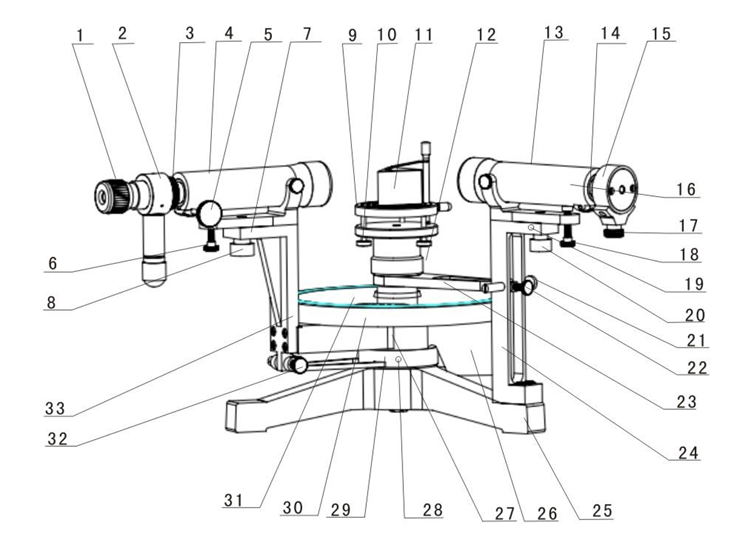
\includegraphics[width=0.8\textwidth]{Fig/屏幕截图 2025-11-04 212139.png} % 您询问的命令
    \caption{分光计示意图} % 为图片添加编号和标题
    \label{fig:ins} % 为图片添加标签，方便在文中用 \ref{fig:my_image} 引用
    \end{figure}
    \item \textbf{汞灯}：发射包含多条特征波长谱线的多色光源，作为“已知波长标准源”，用于光栅常量标定、未知波长测定等实验环节。
    \item \textbf{钠灯}：发射波长稳定的单色光源（以钠双线为典型特征），为三棱镜折射率测量等“单色光光学实验”提供光源条件。
    \item \textbf{三棱镜}：由高透光光学材料制成的三棱柱元件，用于研究光的折射规律，通过“最小偏向角测量法”可推导其对不同波长光的折射率。
    \item \textbf{光栅}：具有周期性刻线结构的衍射光学元件，基于光的衍射原理实现光谱分光，可用于光栅常量测量、未知波长测定，还能直观体现“刻线数目与分辨本领的关联”。
    \item \textbf{数字光谱仪}：集成化现代光学测量仪器，具备光谱采集、数据处理与分析功能，配套的光纤传输系统是光信号传输的关键部件。
\end{enumerate}

\noindent \textbf{注意事项}：
\begin{enumerate}
    \item 数字光谱仪属于精密设备，需轻拿轻放；其附带的光纤为易碎光学元件，允许适度弯曲但\textbf{严禁折叠}，否则会造成光纤断裂、光信号传输中断。
    \item 汞灯、钠灯属于气体放电光源，电极寿命受开关次数影响极大，实验中应避免频繁通电、关闭，需提前规划好光源的持续使用时段。
\end{enumerate}

\section{实验原理}
\subsection{三棱镜最小偏向角}
如图\ref{fig:prism_refraction}所示，棱镜是由透明介质制成的柱状物体，其截面通常为等腰三角形，故又称三棱镜。当一束光从棱镜一侧入射时，会在第一界面发生折射；折射光在棱镜内部传输一段距离后，会在第二界面再次折射并出射。

\begin{figure}[htbp]
    \centering
    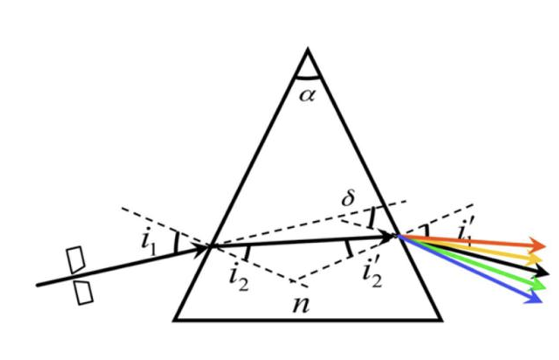
\includegraphics[width=0.8\textwidth]{Fig/屏幕截图 2025-11-04 212204.png} % 请替换为实际图像路径，若无图可保留此占位符
    \caption{棱镜及棱镜中光的折射示意图}
    \label{fig:prism_refraction}
\end{figure}

\subsubsection{偏折角的推导}
经过两次折射后，光线的总偏折角\(\delta\)可通过角度关系推导：
\[
\delta = (i_1 - i_2) + (i_1' - i_2') = (i_1 + i_1') - (i_2 + i_2') \tag{1}
\]
其中，\(i_1\)为第一界面的入射角，\(i_2\)为第一界面的折射角，\(i_2'\)为第二界面的入射角，\(i_1'\)为第二界面的折射角。

考虑棱镜的顶角\(\alpha\)满足几何关系\(\alpha = i_2 + i_2'\)，将其代入式\((1)\)可得偏折角的简化形式：
\[
\delta = (i_1 + i_1') - \alpha \tag{2}
\]

\subsubsection{最小偏向角的条件与公式}
偏折角\(\delta\)与棱镜顶角\(\alpha\)、介质折射率\(n\)及入射角\(i_1\)相关。当棱镜的\(\alpha\)和\(n\)确定后，\(\delta\)仅由\(i_1\)决定。通过改变\(i_1\)（即转动棱镜相对入射光的角度），可发现\(\delta\)存在最小值——最小偏向角\(\delta_m\)。

从物理对称性分析，最小偏向角出现的条件为：
\[
i_1 = i_1',\quad i_2 = i_2' \tag{3}
\]

此时，最小偏向角\(\delta_m\)、顶角\(\alpha\)和折射率\(n\)满足如下核心公式：
\[
n = \frac{\sin\frac{\alpha + \delta_m}{2}}{\sin\frac{\alpha}{2}} \tag{4}
\]

\subsubsection{应用：测量材料折射率}
利用式\((4)\)，可将待测材料制成已知顶角\(\alpha\)的三棱镜，通过实验测量其最小偏向角\(\delta_m\)，进而计算出材料的折射率\(n\)，这是光学中测量透明介质折射率的经典方法之一。

\subsection{光栅原理}
光栅是重要的分光元件，可将入射光中不同波长的光分离，是光谱分析的核心工具之一。衍射光栅主要分为透射光栅和反射光栅两类，实验中常用的平面透射光栅等效于一组数量众多、排列紧密且均匀的平行狭缝阵列。

\subsubsection{夫琅禾费衍射与光栅方程}
根据夫琅禾费衍射理论，平行光入射光栅时，每条狭缝产生衍射，各狭缝的衍射光间会发生干涉。仅当衍射角满足特定条件时，光强会增强形成亮纹。

\paragraph{垂直入射时的光栅方程}
当平行光垂直投射到光栅平面时，光栅方程为：
\[
d \sin\theta = k\lambda, \quad k = 0, \pm1, \pm2, \dots \tag{4}
\]
其中：
- \(\theta\) 为衍射角（衍射光与光栅法线的夹角）；
- \(\lambda\) 为光波波长；
- \(k\) 为光谱级数（\(k=0\) 对应零级谱线，\(k=\pm1,\pm2,\dots\) 对应正负各级谱线）；
- \(d\) 为缝距（相邻狭缝对应点的距离，又称光栅常量），其倒数 \(1/d\) 为光栅空间频率。

满足该式时，干涉相长，对应方向光强增强；其余方向光强几乎完全抵消。

\paragraph{斜入射时的光栅方程}
当入射光不与光栅表面垂直时，设入射光与光栅法线的夹角为 \(i\)，光栅方程修正为：
\[
d \sin(\theta - i) = k\lambda, \quad k = 0, \pm1, \pm2, \dots \tag{5}
\]

\subsubsection{衍射谱线的形成}
若用会聚透镜将衍射后的平行光会聚，在透镜后焦面上会呈现一系列亮线（谱线）。这些谱线沿垂直于光栅刻线的方向展开，具有以下特点：

当平行光管产生的平行光垂直入射光栅时，透镜后焦面的谱线分布如图\ref{fig:grating_diffraction}所示：
- \(\theta = 0\) 方向出现中央极强（零级谱线）；
- \(\pm1\)、\(\pm2\) 等各级谱线对称分布在零级谱线两侧。

\begin{figure}[htbp]
    \centering
    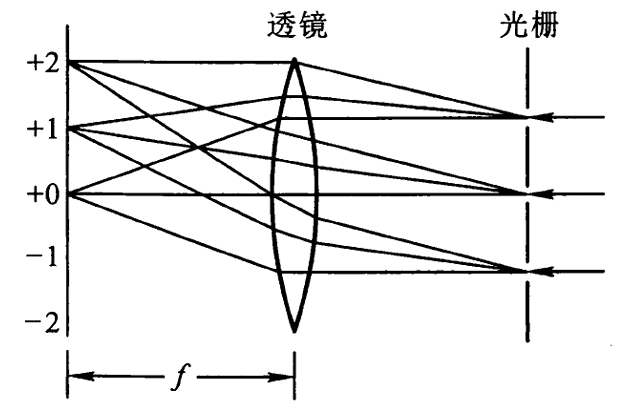
\includegraphics[width=0.8\textwidth]{Fig/屏幕截图 2025-11-04 212211.png} 
    \caption{衍射光栅原理示意图}
    \label{fig:grating_diffraction}
\end{figure}

\subsubsection{光栅衍射光谱与应用}
若光源含多种波长的光，同一级谱线（同一 \(k\)）会因波长不同而具有不同衍射角 \(\theta\)。因此，在透镜焦面上会按波长次序和谱线级次排列，从第0级开始，左右两侧由短波向长波依次分布，形成光栅衍射光谱。

光栅衍射的核心应用包括：
\begin{itemize}
    \item 已知 \(\lambda\) 和 \(k\)，测量衍射角 \(\theta\)，可通过光栅方程计算光栅常量 \(d\)；
    \item 已知 \(d\) 和 \(k\)，测量衍射角 \(\theta\)，可求得未知光波的波长 \(\lambda\)（光谱分析的关键原理）。
\end{itemize}

\subsection{光栅光谱仪}
光栅光谱仪是以光栅为色散元件的分光仪器，具备产生单色光、分析光源光谱、测量材料光谱特性等功能，是光谱分析领域应用最广泛的仪器之一，在光学检测、材料分析、天体物理等领域具有关键地位。

\subsubsection{Czerny-Turner型（C-T型）光栅光谱仪的光路原理}
图\ref{fig:CT_grating_spectrometer}展示了典型Czerny-Turner型（简称C-T型）光栅光谱仪的光学原理图，其光路因结构简单、对称且扫面线性的特点，被工业与科研领域广泛采用。

\begin{figure}[htbp]
    \centering
    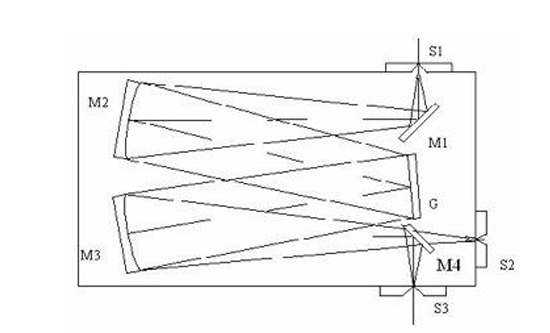
\includegraphics[width=0.8\textwidth]{Fig/屏幕截图 2025-11-04 212219.png} % 请替换为实际图像文件路径
    \caption{典型Czerny-Turner型光栅光谱仪光学原理图}
    \label{fig:CT_grating_spectrometer}
\end{figure}

其工作流程与组件功能可分为以下三个核心环节：
\begin{enumerate}
    \item \textbf{入射与准直系统}：入射光聚焦于\(\text{S1}\)（入射狭缝）平面，形成窄缝型光束；经平面反射镜\(\text{M1}\)转向后，由凹面反射镜\(\text{M2}\)（准光镜）进行准直——由于\(\text{M2}\)到\(\text{S1}\)的距离等于其焦距，因此出射光为平行光束，为后续衍射色散提供了必要的平行光条件。
    \item \textbf{色散系统}：平行光束入射平面衍射光栅\(\text{G}\)后，不同波长的光因光栅衍射效应满足光栅方程 \(d\sin\theta = k\lambda\)（\(d\)为光栅常量，\(\theta\)为衍射角，\(k\)为光谱级数，\(\lambda\)为波长），从而被色散为不同方向的平行光束，实现了波长的空间分离。
    \item \textbf{成像与探测系统}：色散后的平行光束经凹面反射镜\(\text{M3}\)（物镜）反射并聚焦于出射平面，形成光谱；\(\text{S2}\)（出射狭缝）仅允许某一波长的单色光通过，最终由探测组件（如\(\text{S3}\)处的CCD或\(\text{S2}\)处的光电倍增管）完成光信号的接收与转换。通过转动光栅\(\text{G}\)改变衍射角，可筛选出不同波长的单色光，实现光谱的扫描与分析。
\end{enumerate}

图中各组件的定义为：\(\text{M1}\)（平面反射镜）、\(\text{M2}\)（准光镜，凹面反射镜）、\(\text{M3}\)（物镜，凹面反射镜）、\(\text{M4}\)（平面反射镜）、\(\text{G}\)（平面衍射光栅）；\(\text{S1}\)（入射狭缝）、\(\text{S2}\)（光电倍增管接收狭缝）、\(\text{S3}\)（CCD接收狭缝）。

\section{实验操作}
\subsection{分光计整体校准与实验关键问题解析}

分光计是光学角度精密测量的核心仪器，其校准质量直接决定后续三棱镜最小偏向角测定、光栅衍射光谱分析等实验的测量精度。校准的核心目标可概括为以下三点：
\begin{enumerate}[label=(\arabic*)]
    \item 平行光管出射严格平行光；
    \item 望远镜聚焦于无穷远（能稳定接收平行光）；
    \item 望远镜光轴、平行光管光轴及载物平台均与仪器中心转轴垂直。
\end{enumerate}
以下结合校准原理、分步操作，重点解析实验中易出现的问题、异常现象及解决方案。

\subsubsection{校准核心原理与实验意义}
分光计的测量本质是“平行光入射-光学元件（棱镜/光栅）色散/折射-平行光接收”的光路闭环。若校准不达标，会引入系统性误差：
\begin{itemize}
    \item 平行光管未出射平行光或望远镜未聚焦于无穷远：导致衍射/折射光的传播路径偏离理论模型，出现谱线模糊、视差等现象；
    \item 光轴与中心转轴不垂直：引入“偏心差”，使测量角度与实际角度偏差可达$1^\circ\sim3^\circ$，严重影响实验数据有效性；
    \item 载物台不水平：放置光学元件后会导致其工作面倾斜，破坏入射光与元件表面的几何关系，无法观察到预期的反射像或谱线。
\end{itemize}
因此，校准环节是实验成功的前提，需遵循“粗调打底、细调逐次逼近”的原则，避免盲目操作。

\subsubsection{分步校准操作与实验问题深度解析}

\paragraph{粗调（目视预调节）}
\textbf{操作细节}：
\begin{enumerate}[label=(\arabic*), itemsep=0.5ex]
    \item 调节望远镜仰角调节螺丝（位于望远镜镜筒下方）、平行光管仰角调节螺丝，使二者镜筒大致水平（可通过目视镜筒轴线判断）；
    \item 调节载物台下方三个调平螺丝（记为$S_1$、$S_2$、$S_3$），使载物台表面与底座大致平行（可将水平仪置于载物台中心辅助判断，无水平仪时可通过“目测载物台边缘与底座距离均匀”粗略判断）；
    \item 转动望远镜，使其光轴大致对准平行光管出口，确保二者轴线初步共线。
\end{enumerate}

\textbf{实验常见问题与解决方案}：
\begin{description}
    \item[问题1：] 粗调时未关注载物台水平，导致后续反射像难以找到。\\
    \textbf{现象：} 将双面反射镜置于载物台后，转动载物台始终无绿色十字反射像。\\
    \textbf{解决方案：} 重新调节载物台三个调平螺丝，使载物台“微倾但不歪斜”，同时小幅度转动望远镜，扩大搜索范围；若仍无像，需检查反射镜是否紧贴载物台（避免镜面倾斜过度）。
    
    \item[问题2：] 平行光管与望远镜轴线偏差过大。\\
    \textbf{现象：} 目视可见二者镜筒明显错位，即使粗调后也无法通过望远镜观察到平行光管的光斑。\\
    \textbf{解决方案：} 松开望远镜锁紧螺丝，平移或转动望远镜，直至镜筒轴线与平行光管出口中心对齐，再锁紧螺丝。
\end{description}

\paragraph{调节望远镜聚焦于无穷远（消除视差）}
\textbf{核心目标：} 使望远镜的分划板位于其物镜的焦平面上，确保接收的平行光能在分划板上形成清晰无视差的像。

\textbf{操作步骤}：
\begin{enumerate}[label=(\arabic*), itemsep=0.5ex]
    \item 接通望远镜内置照明电源（绿色十字光源），将双面反射镜平置于载物台中心，使反射镜镜面与载物台任意两个调平螺丝（如$S_1$、$S_2$）的连线垂直（此时$S_3$可单独调节镜面倾斜角度）；
    \item 缓慢转动载物台（每次转动$5^\circ\sim10^\circ$），同时通过望远镜目镜观察，直至看到模糊的绿色十字光斑（反射像）；
    \item 旋转望远镜调焦手轮（位于目镜外侧），使绿色十字像逐渐清晰；随后左右移动眼睛，观察十字像与分划板黑叉丝是否存在相对位移（即“视差”），若有视差，微调调焦手轮直至视差完全消除——此时望远镜已聚焦于无穷远。
\end{enumerate}

\begin{figure}[htbp]
    \centering
    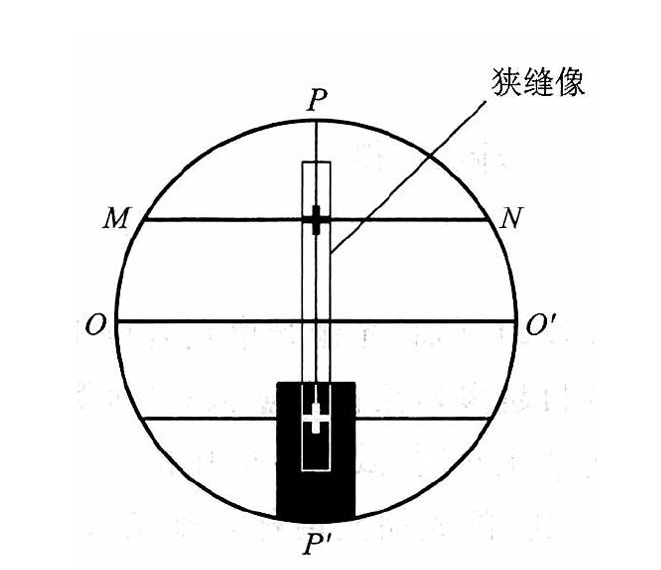
\includegraphics[width=0.35\textwidth]{Fig/屏幕截图 2025-11-04 212225.png}
    \caption{望远镜分划板与绿色十字反射像示意图（无视差状态）}
    \label{fig:reticle}
\end{figure}

\textbf{实验常见问题与解决方案}：
\begin{description}
    \item[问题1：] 始终无法观察到绿色十字反射像。\\
    \textbf{可能原因：} 
    \begin{enumerate*}[label=(\arabic*)]
        \item 反射镜镜面未对准望远镜；
        \item 望远镜照明电源未接通或亮度不足；
        \item 粗调时仰角偏差过大。
    \end{enumerate*}\\
    \textbf{解决方案：} 
    \begin{enumerate*}[label=(\arabic*)]
        \item 转动载物台的同时，小幅度调节望远镜仰角螺丝；
        \item 检查电源接口是否插紧，增大光源亮度；
        \item 重新进行粗调，确保反射镜与望远镜轴线夹角不超过$10^\circ$。
    \end{enumerate*}
    
    \item[问题2：] 十字像清晰但存在明显视差。\\
    \textbf{现象：} 眼睛左右移动时，绿色十字像与黑叉丝沿水平或竖直方向错位。\\
    \textbf{危害：} 视差会导致后续角度读数时的主观误差，严重时偏差可达$0.5^\circ$。\\
    \textbf{解决方案：} 采用“双向调焦法”——先顺时针旋转调焦手轮至像模糊，再逆时针缓慢旋转至清晰，反复2$\sim$3次，直至视差完全消除。
\end{description}

\paragraph{调节望远镜光轴与中心转轴垂直（各半调节法）}
\textbf{核心原理：} 利用双面反射镜的对称性，通过“逐次逼近”消除望远镜光轴与转轴的倾斜偏差，是校准中最关键的步骤。

\textbf{操作步骤}：
\begin{enumerate}[label=(\arabic*), itemsep=0.5ex]
    \item 当望远镜中出现清晰无视差的绿色十字像后，观察其与分划板上“上十字丝”（标准对准位置）的垂直距离（记为$\Delta h$）；
    \item 调节载物台调平螺丝（对应反射镜所在侧的螺丝，如$S_1$），使十字像向标准位置移动$\Delta h/2$（消除一半偏差）；
    \item 调节望远镜仰角调节螺丝，使十字像与上十字丝完全重合（消除剩余一半偏差）；
    \item 将载物台旋转$180^\circ$，使反射镜另一面对准望远镜，此时会观察到十字像再次偏离标准位置（因光轴与转轴仍有微小偏差）；
    \item 重复步骤(2)$\sim$(4)，直至载物台旋转$180^\circ$前后，绿色十字像均能与上十字丝完全重合——此时望远镜光轴与中心转轴垂直。
\end{enumerate}

\textbf{实验常见问题与解决方案}：
\begin{description}
    \item[问题1：] 旋转$180^\circ$后反射像消失。\\
    \textbf{现象：} 第一次对准反射镜时能看到像，旋转$180^\circ$后完全无像。\\
    \textbf{可能原因：} 粗调时载物台或望远镜仰角偏差过大，导致反射镜另一面对准望远镜时，反射光无法进入镜筒。\\
    \textbf{解决方案：} 回到粗调步骤，重新调节载物台水平和望远镜仰角，确保反射镜两面均能大致对准望远镜；若仍无像，可将反射镜旋转$90^\circ$后再试。
    
    \item[问题2：] 调节后偏差反复，无法收敛。\\
    \textbf{现象：} 每次调节后十字像接近标准位置，但旋转$180^\circ$后偏差反而增大。\\
    \textbf{原因：} 调节幅度过大，破坏了“各半调节”的逐次逼近逻辑。\\
    \textbf{解决方案：} 采用“小幅度调节”——每次调节螺丝仅旋转$1/8$圈，逐次缩小偏差；同时记录调节方向，避免反向操作。
\end{description}

\paragraph{调节平行光管（出射平行光且光轴与转轴垂直）}
\textbf{核心目标：} 使平行光管的狭缝位于其物镜的焦平面上（出射平行光），且光轴与望远镜光轴平行（即与转轴垂直）。

\textbf{操作步骤}：
\begin{enumerate}[label=(\arabic*), itemsep=0.5ex]
    \item 移走载物台上的双面反射镜，将望远镜正对平行光管，打开平行光管光源（如钠灯、汞灯）；
    \item 松开平行光管狭缝锁紧螺丝（位于狭缝套管侧面），前后移动狭缝套管，直至望远镜中观察到清晰的狭缝像，且左右移动眼睛时，狭缝像与分划板叉丝无视差（此时狭缝位于平行光管物镜焦平面，出射平行光）；
    \item 调节狭缝宽度调节螺丝（位于平行光管前端），使狭缝像宽度约为$0.1\sim0.2\ \text{mm}$（过宽会导致后续角度测量分辨率下降，过窄则光强不足）；
    \item 旋转狭缝套管，使狭缝像呈竖直方向（与分划板竖直叉丝平行）；
    \item 调节平行光管仰角调节螺丝，使竖直狭缝像的中心与分划板中央水平叉丝重合——此时平行光管光轴与望远镜光轴平行，即与中心转轴垂直。
\end{enumerate}

\textbf{实验常见问题与解决方案}：
\begin{description}
    \item[问题1：] 狭缝像模糊或无法聚焦。\\
    \textbf{现象：} 移动狭缝套管时，狭缝像始终呈弥散状，无清晰边缘。\\
    \textbf{可能原因：} 狭缝被灰尘堵塞，或套管移动范围未覆盖物镜焦平面。\\
    \textbf{解决方案：} 用镜头纸轻轻擦拭狭缝（避免刮伤）；松开狭缝锁紧螺丝，扩大套管移动范围（注意不要用力过猛导致套管脱落）。
    
    \item[问题2：] 狭缝像倾斜，无法与竖直叉丝平行。\\
    \textbf{现象：} 旋转狭缝套管时，狭缝像始终倾斜，影响后续谱线角度测量的准确性。\\
    \textbf{原因：} 狭缝套管与平行光管轴线不共线，或狭缝本身存在形变。\\
    \textbf{解决方案：} 松开狭缝套管的固定螺丝，微调套管的安装角度，直至狭缝像与竖直叉丝完全平行后再锁紧。
\end{description}

\subsubsection{校准完成的判定标准}
校准合格需同时满足以下4个条件，方可开展后续实验：
\begin{enumerate}[label=(\arabic*), itemsep=0.3ex]
    \item 望远镜：聚焦于无穷远，分划板十字丝与反射像无视差；
    \item 光轴垂直：载物台旋转$180^\circ$前后，双面反射镜的反射像均与上十字丝重合；
    \item 平行光管：出射平行光，狭缝像清晰无视差，宽度合适且竖直；
    \item 光轴平行：平行光管狭缝像的中心与分划板中央叉丝重合，与望远镜光轴共线。
\end{enumerate}
若校准后仍存在微小偏差，可在后续实验中通过“多次测量取平均值”或“对称读数法”（消除偏心差）进一步减小误差。

\subsection{测量三棱镜的基本参数}
三棱镜的顶角与最小偏向角是表征其光学特性的核心参数，通过分光计测量可进一步推导材料折射率。以下从操作步骤、原理分析、实验问题及数据处理等维度，系统阐述测量方法。

\subsubsection{放置三棱镜}
将三棱镜置于载物台时，需确保\textbf{三个顶点分别位于载物台三个调平螺丝构成的三角形三边上}。此布局的优势在于：每个调平螺丝可独立调节三棱镜的一个光学面（如\(AB\)面、\(AC\)面），为后续"主截面与转轴垂直"的调节提供操作自由度。

\textbf{实验注意事项}：
\begin{itemize}
    \item 轻拿轻放棱镜，避免划伤光学面或破坏载物台水平；
    \item 保证棱镜底面与载物台贴合紧密，若存在缝隙，需微调调平螺丝修正。
\end{itemize}

\subsubsection{调节棱镜主截面与仪器转轴垂直}
棱镜的\textbf{主截面}是指与底面垂直的截面（两光学面的交线所在平面）。调节目标是使主截面与分光计中心转轴垂直，确保后续角度测量的几何关系严格满足理论模型。

\textbf{操作步骤（各半调节法）}：
\begin{enumerate}[label=(\arabic*), itemsep=0.5ex]
    \item 转动载物台，使棱镜\(AB\)面对准望远镜；
    \item 仅调节载物台对应\(AB\)面的调平螺丝，通过“各半调节法”（每次消除十字像与分划板标准位置垂直距离的一半），使\(AB\)面反射的绿色十字像落于标准位置；
    \item 转动载物台，使\(AC\)面对准望远镜，重复步骤(2)，调节对应调平螺丝；
    \item 反复迭代步骤(2)~(3)，直至\(AB\)、\(AC\)面反射的绿色十字像均能稳定落于标准位置。
\end{enumerate}

\textbf{实验常见问题与解决方案}：
\begin{description}
    \item[问题1：] 调节后十字像偏离无规律。\\
    \textbf{原因：} 误判调平螺丝与光学面的对应关系。\\
    \textbf{解决方案：} 标记每个螺丝对应的光学面，重新逐一调节。
    
    \item[问题2：] 某一光学面无反射像。\\
    \textbf{原因：} 光学面与望远镜光轴夹角过大。\\
    \textbf{解决方案：} 微调载物台和望远镜仰角，扩大反射光接收范围后再进行"各半调节"。
\end{description}

\subsubsection{测量顶角\(A\)（两种高精度方法）}
顶角\(A\)是三棱镜两光学面（\(AB\)与\(AC\)）的夹角，以下两种方法可有效消除系统误差。

\paragraph{自准直法}
\textbf{原理}：利用望远镜自准直功能，通过测量望远镜对准两光学面的角度差推导顶角。

\textbf{操作步骤}：
\begin{enumerate}[label=(\arabic*), itemsep=0.5ex]
    \item 点亮望远镜照明光源，对准\(AB\)面，使绿色十字像与分划板上方叉丝重合，记录双游标读数\(\theta_1\)、\(\theta_1'\)；
    \item 转动望远镜对准\(AC\)面，重复步骤(1)，记录读数\(\theta_2\)、\(\theta_2'\)；
    \item 按公式计算顶角：
\[
A = 180^\circ - \frac{|\left(\theta_2 - \theta_1\right) + \left(\theta_2' - \theta_1'\right)|}{2}
\]
\end{enumerate}

\textbf{原理补充}：望远镜转动角度为\(180^\circ - A\)，双游标读数平均可消除\textbf{偏心差}（分光计转轴与刻度盘中心不重合的误差）。

\paragraph{反射法}
\textbf{原理}：利用平行光管的平行光入射，经两光学面反射后，通过反射光角度差推导顶角。

\textbf{操作步骤}：
\begin{enumerate}[label=(\arabic*), itemsep=0.5ex]
    \item 点亮平行光管光源，将三棱镜置于载物台中心，顶角\(A\)对准平行光管；
    \item 转动望远镜至位置\(I\)，接收\(AB\)面反射狭缝像，记录读数；
    \item 转动望远镜至位置\(II\)，接收\(AC\)面反射狭缝像，记录读数；
    \item 顶角\(A = \frac{|\text{位置}II - \text{位置}I|}{2}\)。
\end{enumerate}

\textbf{方法对比}：
\begin{itemize}
    \item 自准直法操作简洁，适合快速测量；
    \item 反射法精度更高，受平行光均匀性影响小；
    \item 建议两种方法各测3次，取平均值减小随机误差。
\end{itemize}

\subsubsection{测量最小偏向角\(\delta_m\)}
最小偏向角是三棱镜色散特性的关键指标，其测量核心是识别"谱线反向的转折点"。

\paragraph{寻找折射光（粗定位）}
\begin{enumerate}[label=(\arabic*), itemsep=0.5ex]
    \item 移开三棱镜，将望远镜与平行光管共轴，记录入射光方向的双游标读数\(\varphi_0\)、\(\varphi_0'\)；
    \item 放回三棱镜，使入射光在\(AC\)面入射、\(AB\)面出射，用眼睛在出射光方向寻找彩色谱线（如钠光黄线、汞灯绿线）；
    \item 缓慢转动载物台，同时用望远镜跟踪谱线，观察其移动趋势。
\end{enumerate}

\textbf{物理本质}：谱线移动源于偏向角\(\delta\)随入射角的变化，转动载物台会改变入射光在\(AC\)面的入射角，进而改变出射光的偏向角。

\paragraph{精确确定最小偏向角位置（转折点识别）}
当载物台转动到某一位置时，谱线会\textbf{停止移动并反向偏转}，此"转折点"即为最小偏向角位置。

\textbf{操作技巧}：
\begin{itemize}
    \item 载物台转动需极缓慢，同时微调望远镜方位，确保叉丝始终跟踪谱线；
    \item 采用"双向逼近法"：先顺时针转至谱线反向，再逆时针转至反向，取中间位置提高精度。
\end{itemize}

\textbf{实验常见问题与解决方案}：
\begin{description}
    \item[问题1：] 谱线无反向，单向移动。\\
    \textbf{原因：} 三棱镜放置方向错误或载物台转动方向错误。\\
    \textbf{解决方案：} 重新确认入射面与入射光的几何关系，调整载物台转动方向。
    
    \item[问题2：] 转折点模糊，谱线边缘不清晰。\\
    \textbf{原因：} 光源单色性差或狭缝过宽。\\
    \textbf{解决方案：} 使用单色光源（如钠灯）并调窄狭缝（\(0.1\ \text{mm}\)左右）。
\end{description}

\paragraph{测量出射光方向与计算最小偏向角}
当叉丝精确对准最小偏向角处的谱线时，记录双游标读数\(\varphi_1\)、\(\varphi_1'\)，按公式计算：
\[
\delta_m = \frac{|\left(\varphi_1 - \varphi_0\right) + \left(\varphi_1' - \varphi_0'\right)|}{2}
\]

\subsubsection{计算折射率\(n\)}
结合顶角\(A\)和最小偏向角\(\delta_m\)，代入光学公式：
\[
n = \frac{\sin\frac{A + \delta_m}{2}}{\sin\frac{A}{2}}
\]
对于钠光（\(\lambda = 589.3\ \text{nm}\)），可计算出三棱镜玻璃的折射率。

\textbf{数据处理建议}：
\begin{itemize}
    \item 顶角\(A\)和最小偏向角\(\delta_m\)各测3次以上，取平均值；
    \item 计算时注意角度单位统一，使用计算器三角函数功能确保精度。
\end{itemize}

\subsection{测量光栅基本参数}
光栅衍射实验中，准确测量光栅常数、谱线波长等基本参数的前提是对光栅进行精确调节，并采用科学的测量方法消除系统误差。以下从\textbf{光栅调节}与\textbf{衍射角及光栅参数测量}两方面展开详细说明。

\subsubsection{光栅的调节}
光栅调节的核心是确保"光栅平面垂直于望远镜光轴"且"光栅刻痕与仪器转轴平行"，这是获得对称、清晰衍射谱线的基础。

\paragraph{1. 放置光栅}
将光栅小心放置于分光计载物台上，为简化后续调节，需使光栅平面\textbf{垂直于载物台下任意两个调平螺丝的连线}——此时第三个调平螺丝可单独控制光栅平面的倾斜度。
\textit{实验注意}：操作时需保持光栅表面清洁，避免指纹、灰尘影响反射与衍射效果。

\paragraph{2. 调节光栅平面垂直于望远镜光轴（自准直法）}
点亮望远镜照明灯，转动望远镜使其对准光栅平面，观察光栅平面反射的\textbf{绿色十字像}；调节载物台调平螺丝（\textbf{严禁调节望远镜仰角螺丝}），使绿色十字像与分划板上方的标准位置重合。
\textit{实验现象与问题分析}：
- 若绿色十字像模糊，说明望远镜未聚焦于无穷远，需先完成望远镜的聚焦调节；
- 若转动望远镜时十字像“丢失”，表明光栅平面与望远镜光轴夹角过大，需先粗略调整载物台再细调。
当十字像与标准位置重合时，光栅平面已与仪器转轴平行，即垂直于望远镜光轴。

\paragraph{3. 调节光栅刻痕与转轴平行}
将望远镜转回对准平行光管，使中央零级（\( k=0 \)）狭缝像与分划板竖直叉丝精确重合；随后向左、右转动望远镜，观察\( k=\pm1 \)级衍射谱线。
\textit{实验现象与问题分析}：
若两侧谱线高度不一致（如左侧偏高、右侧偏低），说明光栅刻痕未平行于仪器转轴。此时需调节载物台螺丝，微转光栅方位，直至左右衍射谱线均被分划板中央水平叉丝同时穿过（高度一致）。
此步骤需反复微调——若调节不到位，后续衍射角测量将引入显著系统误差。


\subsubsection{衍射角\(\theta\)与光栅参数的测量}
采用\textbf{对称测量法}测量衍射角，可消除光栅未完全垂直于入射光的系统误差；结合\textbf{光栅方程}可进一步计算光栅常数与未知谱线波长。

\paragraph{对称测量法测量衍射角\(\theta\)}
以汞灯绿光（\( \lambda_{\text{绿}} = 546.1\ \text{nm} \)）的一级衍射为例，步骤如下：

\begin{enumerate}[itemsep=0.5ex]
    \item \textbf{确定零级位置}：将望远镜精确对准中央零级亮纹（最亮、最宽的白色亮线），使狭缝像与分划板竖直叉丝重合，记录两个游标的读数\( \theta_0 \)和\( \theta_0' \)。
    
    \item \textbf{测量正负一级位置}：
        \begin{itemize}
            \item 向左转动望远镜，找到汞灯绿光\( k=+1 \)级衍射谱线，使叉丝竖线对准其中心，记录读数\( \theta_{\text{左}} \)和\( \theta_{\text{左}}' \)；
            \item 向右转动望远镜（越过零级），找到\( k=-1 \)级衍射谱线，对准中心后记录读数\( \theta_{\text{右}} \)和\( \theta_{\text{右}}' \)。
        \end{itemize}
    
    \item \textbf{计算衍射角}：
        \begin{enumerate}[label=\roman*.]
            \item 计算左侧衍射角：\( \phi_{\text{左}} = |\theta_{\text{左}} - \theta_0| \)，\( \phi_{\text{左}}' = |\theta_{\text{左}}' - \theta_0'| \)；
            \item 计算右侧衍射角：\( \phi_{\text{右}} = |\theta_{\text{右}} - \theta_0| \)，\( \phi_{\text{右}}' = |\theta_{\text{右}}' - \theta_0'| \)；
            \item 消除偏心差，取总夹角平均值：\( 4\Phi = (\phi_{\text{左}} + \phi_{\text{右}}) + (\phi_{\text{左}}' + \phi_{\text{右}}') \)，则一级衍射角\( \theta = 2\Phi \)。
        \end{enumerate}
\end{enumerate}

\textbf{误差分析}：游标读数的估读误差、谱线中心对准的偏差属于随机误差；而对称测量法的核心价值是消除了光栅倾斜的系统误差，使\( \theta \)的测量更准确。

\paragraph{光栅常数\( d \)的计算}
根据光栅方程 \( d\sin\theta = k\lambda \)，对于\( k=1 \)级汞灯绿光衍射，将\( \lambda = \lambda_{\text{绿}} = 546.1\ \text{nm} \)和测得的\( \theta \)代入，得：
\[ d = \frac{\lambda_{\text{绿}}}{\sin\theta} \]
光栅常数\( d \)的物理意义是光栅相邻刻痕的间距，单位通常为\( \text{nm} \)或\( \text{mm} \)。

\paragraph{未知光波长\( \lambda \)的计算}
已知光栅常数\( d \)后，换用未知光源（如钠灯）或汞灯的其他谱线（如黄光），重复上述衍射角测量步骤；将测得的\( \theta \)和级数\( k \)代入光栅方程，即可计算未知谱线的波长：
\[ \lambda = \frac{d\sin\theta}{k} \]

\textbf{实验拓展与注意事项}：
\begin{itemize}
    \item 测量多组谱线的波长可验证光栅方程的普适性；
    \item 计算时需注意单位统一（如将角度转换为弧度参与运算）；
    \item 对每条谱线的正负级衍射角均应测量，以进一步减小误差。
\end{itemize}

\subsection{数字光谱仪的光谱测量实验}
\label{subsec:digital-spectrometer}

\subsubsection{实验原理}
数字光谱仪基于\textbf{光学分光与光电探测技术}，将入射光通过内部光栅等光学元件分光后，由光电探测器将不同波长的光信号转换为电信号，经模数转换后传输至计算机，通过专用软件（如Spectra Smart）完成光谱数据的采集、处理与可视化，最终输出光源的波长-光强分布曲线。该技术可实现对光源光谱特性的高精度分析，是光谱学研究、光源质量检测的核心手段之一。

\subsubsection{实验设备}
\begin{itemize}
    \item 便携数字光谱仪（含光纤探测探头）
    \item 工作电脑（预装Spectra Smart软件）
    \item 目标光源组：钠灯、汞灯、H灯、氮灯、手机LED灯（含背光、闪光灯）、手机屏幕、室内照明灯（白炽灯、LED灯等）、日光（晴天/阴天）
\end{itemize}

\subsubsection{操作步骤}
\begin{enumerate}
    \item \textbf{仪器连接与初始化}：将数字光谱仪通过专用接口与工作电脑物理连接，随后取下光纤探头的保护帽（\textbf{关键注意：测量结束后必须及时盖上，防止光纤端面被灰尘污染或机械划伤，否则会导致光谱信号失真}）。启动Spectra Smart软件，新建工作窗口，在软件中完成设备通讯检测，确认光谱仪处于就绪状态。
    \item \textbf{光源对准与初步测量}：手持光纤探头对准目标光源，调整探头与光源的距离、角度（亮光源可适当拉远，弱光源可适当贴近），使光信号能有效耦合进入光纤。
    \item \textbf{积分时间优化设置}：积分时间是光谱仪采集光信号的时长，需根据光源亮度动态调整。若光源过亮（如汞灯、手机屏幕强光），设置过短积分时间（如20–50 ms）可避免“光谱过曝”（光强超出探测器线性范围，谱线顶部被截断）；若光源较暗（如室内弱光、阴天日光），需延长积分时间（如200 ms–5 s）以避免“光谱欠曝”（光强信号微弱，谱线细节丢失）。每次调整后需实时预览光谱，直至获得轮廓清晰、强度合理的光谱曲线。
    \item \textbf{光谱采集与数据保存}：确认积分时间合理后，执行“光谱采集”操作，观察并分析光谱的波长分布、特征峰位置与强度；随后将光谱图（如PNG格式）或原始数据（如CSV格式）保存至指定路径，便于后续分析。
    \item \textbf{多光源系统性测量}：按上述步骤依次对钠灯、汞灯、H灯、氮灯、手机LED灯、手机屏幕、室内照明灯、日光等光源进行测量，分别记录各光源的光谱特征。
\end{enumerate}

\subsubsection{实验现象与分析}
\begin{enumerate}
    \item \textbf{钠灯光谱特征}：钠灯呈现典型的\textbf{黄色双谱线}，中心波长分别为589.0 nm和589.6 nm（钠D双线），谱线尖锐且光强集中。将该结果与光栅衍射实验测得的钠灯波长对比，二者应具有良好一致性，此对比可验证光谱仪的波长测量精度。
    \item \textbf{汞灯光谱特征}：汞灯属于原子发射光谱，表现为多条离散的特征明线，覆盖紫外至可见光区域（如404.7 nm（紫）、435.8 nm（蓝）、546.1 nm（绿）、577.0 nm（黄）等），谱线强度差异显著，可作为光谱仪波长校准的标准参考。
    \item \textbf{人工光源（LED、手机屏幕、室内灯）光谱特征}：
        - 手机LED灯与屏幕：光谱多为“连续谱+窄带特征峰”的组合，冷色温LED蓝光成分占比高，暖色温LED红光成分占比高；手机屏幕光谱还会随显示内容（如红/绿/蓝画面）呈现动态的光谱成分变化。
        - 室内白炽灯：光谱接近连续谱，光强随波长增加先升后降；荧光灯/LED照明灯则常表现为连续谱叠加特定波长的强峰（由荧光粉或LED芯片发光特性决定）。
    \item \textbf{日光光谱特征}：晴天日光光谱接近连续谱，且因大气中氧、水汽的吸收作用存在若干暗线；阴天日光光谱强度整体降低，分布更趋平缓，短波长（蓝光）成分占比相对减少。
    \item \textbf{测量偏差分析}：若光栅实验与光谱仪测得的波长存在偏差，需从三方面排查：光栅常数的测量误差、衍射角的读取误差、光谱仪的系统校准误差（如分光元件的色散非线性、探测器的响应不均匀性）。
\end{enumerate}

\subsubsection{注意事项}
\begin{itemize}
    \item 光纤探头保护帽是维持探头性能的关键部件，装卸时需轻拿轻放，严禁在无保护帽时将探头随意放置。
    \item 测量强光源时（如汞灯、手机闪光灯），单次采集时间不宜过长，且需避免探头长时间直射光源，以防探测器过热损坏。
    \item 软件操作中若出现“设备通讯中断”，需检查硬件连接是否松动，或重启软件与设备后再尝试连接。
\end{itemize}
\section{实验数据}
\subsection{测量三棱镜的基本参数}

\subsubsection{三棱镜顶角}

\paragraph{自准直法测量结果}

原始测量数据及计算结果见表\ref{tab:beta_alpha_data1}。

\begin{table}[htbp]
  \centering
  \caption{自准直法测量数据及顶角$\alpha$计算结果}
  \vspace{0.5em}
  \label{tab:beta_alpha_data1}
  \begin{tabular}{cccccc}
    \toprule
    测量次数 & 光面法线$\beta_1$ & 光面法线$\beta_1'$ & 光面法线$\beta_2$ & 光面法线$\beta_2'$ & 计算值$\alpha$ \\
    \midrule
    1 & $101^\circ5'$ & $281^\circ7'$ & $221^\circ5'$ & $41^\circ7'$ & $60^\circ$ \\
    2 & $259^\circ20'$ & $79^\circ20'$ & $139^\circ25'$ & $319^\circ25'$ & $60^\circ5'$ \\
    \bottomrule
  \end{tabular}
\end{table}

\textbf{计算过程}：

根据公式 $\alpha = 180^\circ - \varphi = 180^\circ - \frac{1}{2}\left[|\beta_1 - \beta_2| + |\beta_1' - \beta_2'|\right]$ 计算$\alpha$及平均值。

\begin{enumerate}[itemsep=0.5ex]
  \item \textbf{测量次数1的$\alpha$计算过程}：
  \begin{itemize}[itemsep=0.3ex]
    \item 计算$|\beta_1 - \beta_2|$：$|101^\circ5' - 221^\circ5'| = 120^\circ$（差值小于$180^\circ$，直接取）
    \item 计算$|\beta_1' - \beta_2'|$：$|281^\circ7' - 41^\circ7'| = 240^\circ$，取最小差值（$360^\circ - 240^\circ = 120^\circ$）
    \item 计算$\varphi$：$\varphi = \frac{1}{2}\left(120^\circ + 120^\circ\right) = 120^\circ$
    \item 计算$\alpha$：$\alpha_1 = 180^\circ - 120^\circ = 60^\circ = 60^\circ0'$（统一为度分形式，便于平均计算）
  \end{itemize}

  \item \textbf{测量次数2的$\alpha$计算过程}：
  \begin{itemize}[itemsep=0.3ex]
    \item 计算$|\beta_1 - \beta_2|$：$|259^\circ20' - 139^\circ25'| = 119^\circ55'$（差值小于$180^\circ$，直接取）
    \item 计算$|\beta_1' - \beta_2'|$：$|79^\circ20' - 319^\circ25'| = 240^\circ5'$，取最小差值（$360^\circ - 240^\circ5' = 119^\circ55'$）
    \item 计算$\varphi$：$\varphi = \frac{1}{2}\left(119^\circ55' + 119^\circ55'\right) = 119^\circ55'$
    \item 计算$\alpha$：$\alpha_2 = 180^\circ - 119^\circ55' = 60^\circ5'$
  \end{itemize}

  \item \textbf{$\alpha$平均值$\bar{\alpha}$计算过程}：
  \begin{itemize}[itemsep=0.3ex]
    \item 角度单位统一：由于$1^\circ = 60'$，先将$\alpha_1$和$\alpha_2$转换为"分"进行计算
      \begin{itemize}
        \item $\alpha_1 = 60^\circ0' = 60 \times 60' + 0' = 3600'$
        \item $\alpha_2 = 60^\circ5' = 60 \times 60' + 5' = 3605'$
      \end{itemize}
    \item 计算总合：$3600' + 3605' = 7205'$
    \item 计算平均值（测量次数$n=2$）：$\bar{\alpha}_{\text{分}} = \frac{7205'}{2} = 3602.5'$
    \item 转换回度分秒形式：$3602.5' = 60^\circ + 2.5'$，其中$0.5' = 0.5 \times 60'' = 30''$，即$\bar{\alpha} = 60^\circ2'30''$（或简写为$60^\circ2.5'$）
  \end{itemize}
\end{enumerate}

\paragraph{自准直法测量结果}

原始测量数据及计算结果见表\ref{tab:beta_alpha_data}。

\begin{table}[htbp]
  \centering
  \caption{反射法测量数据及顶角$\alpha$计算结果}
  \vspace{0.5em}
  \label{tab:beta_alpha_data}
  \begin{tabular}{cccccc}
    \toprule
    测量次数 & 光面法线$\beta_1$ & 光面法线$\beta_1'$ & 光面法线$\beta_2$ & 光面法线$\beta_2'$ & 计算值$\alpha$ \\
    \midrule
    1 & $256^\circ10'$ & $76^\circ10'$ & $136^\circ05'$ & $316^\circ03'$ & $59^\circ54'$ \\
    2 & $237^\circ05'$ & $57^\circ03'$ & $117^\circ25'$ & $297^\circ24'$ & $60^\circ20'30''$ \\
    \bottomrule
  \end{tabular}
\end{table}

\textbf{计算过程}：

根据公式 $\alpha = 180^\circ - \varphi = 180^\circ - \frac{1}{2}\left[|\beta_1 - \beta_2| + |\beta_1' - \beta_2'|\right]$ 计算$\alpha$及平均值。

\begin{enumerate}[itemsep=0.5ex, labelsep=0.5em]
  \item \textbf{测量次数1的$\alpha$计算过程}：
  \begin{itemize}[itemsep=0.3ex, leftmargin=1.5em]
    \item 计算$|\beta_1 - \beta_2|$：$|256^\circ10' - 136^\circ05'| = 120^\circ05'$（差值小于$180^\circ$，直接取）
    \item 计算$|\beta_1' - \beta_2'|$：$|76^\circ10' - 316^\circ03'| = 239^\circ53'$，取最小差值（$360^\circ - 239^\circ53' = 120^\circ07'$）
    \item 计算$\varphi$：$\varphi = \frac{1}{2}\left(120^\circ05' + 120^\circ07'\right) = 120^\circ06'$
    \item 计算$\alpha$：$\alpha_1 = 180^\circ - 120^\circ06' = 59^\circ54'$（统一为度分形式，便于平均计算）
  \end{itemize}

  \item \textbf{测量次数2的$\alpha$计算过程}：
  \begin{itemize}[itemsep=0.3ex, leftmargin=1.5em]
    \item 计算$|\beta_1 - \beta_2|$：$|237^\circ05' - 117^\circ25'| = 119^\circ40'$（差值小于$180^\circ$，直接取）
    \item 计算$|\beta_1' - \beta_2'|$：$|57^\circ03' - 297^\circ24'| = 240^\circ21'$，取最小差值（$360^\circ - 240^\circ21' = 119^\circ39'$）
    \item 计算$\varphi$：$\varphi = \frac{1}{2}\left(119^\circ40' + 119^\circ39'\right) = 119^\circ39'30''$
    \item 计算$\alpha$：$\alpha_2 = 180^\circ - 119^\circ39'30'' = 60^\circ20'30''$
  \end{itemize}

  \item \textbf{$\alpha$平均值$\bar{\alpha}$计算过程}：
  \begin{itemize}[itemsep=0.3ex, leftmargin=1.5em]
    \item 角度单位统一：由于$1^\circ = 60'$，先将$\alpha_1$和$\alpha_2$转换为"分"进行计算
      \begin{itemize}[leftmargin=1em, itemsep=0.2ex]
        \item $\alpha_1 = 59^\circ54' = 59 \times 60' + 54' = 3594'$
        \item $\alpha_2 = 60^\circ20'30'' = 60 \times 60' + 20.5' = 3620.5'$
      \end{itemize}
    \item 计算总合：$3594' + 3620.5' = 7214.5'$
    \item 计算平均值（测量次数$n=2$）：$\bar{\alpha}_{\text{分}} = \frac{7214.5'}{2} = 3607.25'$
    \item 转换回度分秒形式：$3607.25' = 60^\circ + 7.25'$，其中$0.25' = 0.25 \times 60'' = 15''$，即$\bar{\alpha} = 60^\circ7'15''$（或简写为$60^\circ7.25'$）
  \end{itemize}
\end{enumerate}

\paragraph{测量结果}

根据表\ref{tab:beta_alpha_data1}和\ref{tab:beta_alpha_data}中的数据，第一次测量得到的顶角$\alpha_1 = 59^\circ54'$，第二次测量得到的顶角$\alpha_2 = 60^\circ20'30''$。经过计算，得到的平均值为$\bar{\alpha} = 60^\circ7'15''$（或简写为$60^\circ7.25'$）。

\subsubsection{三棱镜最小偏向角}
\begin{table}[htbp]
  \centering
  \caption{最小偏向角测量数据}
  \vspace{0.5em}
  \begin{tabular}{c c c c c}
    \toprule
    测量次数 & 光面法线$\beta_1$ & 光面法线$\beta_1'$ & 光面法线$\beta_2$ & 光面法线$\beta_2'$ \\
    \midrule
    1 & $196^\circ25'$ & $16^\circ25'$ & $145^\circ20'$ & $325^\circ20'$ \\
    2 & $217^\circ25'$ & $37^\circ25'$ & $166^\circ20'$ & $346^\circ20'$ \\
    \bottomrule
  \end{tabular}
\end{table}

% 计算过程

\textbf{最小偏向角\(\delta_{\text{min}}\)的计算}：

根据对称测量法，最小偏向角的计算公式为：\(\delta_{\text{min}} = \frac{1}{2}\left[|\beta_1 - \beta_2| + |{\beta_1'}^{\text{对}} - {\beta_2'}^{\text{对}}|\right]\)，其中需要对测量数据进行适当处理。

\paragraph{第一次测量（测量次数1）}

\begin{itemize}[itemsep=0.3ex]
\item 测量值：\(\beta_1 = 196^\circ25'\)，\(\beta_1' = 16^\circ25'\)，\(\beta_2 = 145^\circ20'\)，\(\beta_2' = 325^\circ20'\)
\item 计算\(|\beta_1 - \beta_2| = |196^\circ25' - 145^\circ20'| = 51^\circ5'\)
\item 计算\(|\beta_1' - \beta_2'| = |16^\circ25' - 325^\circ20'|\)，取最小正角度：\(360^\circ - 308^\circ55' = 51^\circ5'\)
\item \(\delta_{\text{min1}} = \frac{1}{2}\left[51^\circ5' + 51^\circ5'\right] = 51^\circ5'\)
\end{itemize}

\paragraph{第二次测量（测量次数2）}

\begin{itemize}[itemsep=0.3ex]
\item 测量值：\(\beta_1 = 217^\circ25'\)，\(\beta_1' = 37^\circ25'\)，\(\beta_2 = 166^\circ20'\)，\(\beta_2' = 346^\circ20'\)
\item 计算\(|\beta_1 - \beta_2| = |217^\circ25' - 166^\circ20'| = 51^\circ5'\)
\item 计算\(|\beta_1' - \beta_2'| = |37^\circ25' - 346^\circ20'|\)，取最小正角度：\(360^\circ - 308^\circ55' = 51^\circ5'\)
\item \(\delta_{\text{min2}} = \frac{1}{2}\left[51^\circ5' + 51^\circ5'\right] = 51^\circ5'\)
\end{itemize}

\paragraph{平均值}

最小偏向角的平均值为：
\[
\delta_{\text{min平均值}} = \frac{51^\circ5' + 51^\circ5'}{2} = 51^\circ5' \approx 51.08^\circ
\]

\subsubsection{三棱镜折射率计算}

根据公式 \(n = \frac{\sin \frac{\delta_{\text{min}} + A}{2}}{\sin \frac{A}{2}}\)，结合测得的最小偏向角 \(\delta_{\text{min}} = 51^\circ5' \approx 51.08^\circ\) 和三棱镜顶角平均值 \(\bar{\alpha} = 60^\circ2'30'' \approx 60.042^\circ\)，计算折射率：

\begin{itemize}[itemsep=0.3ex]
\item 计算分子：\(\sin \frac{\delta_{\text{min}} + A}{2} = \sin \frac{51.08^\circ + 60.042^\circ}{2} = \sin \frac{111.122^\circ}{2} = \sin 55.561^\circ \approx 0.8246\)
\item 计算分母：\(\sin \frac{A}{2} = \sin \frac{60.042^\circ}{2} = \sin 30.021^\circ \approx 0.5003\)
\item 折射率：\(n = \frac{0.8246}{0.5003} \approx 1.648\)
\end{itemize}

因此，三棱镜的折射率为 \(n \approx 1.648\)。

\section{光栅实验}
\subsection{光栅常数测量}

本实验使用汞灯绿光（\(\lambda = 546.1\ \text{nm}\)）的一级衍射谱线，采用对称测量法测量衍射角，进而计算光栅常数\(d\)。

\subsubsection{测量数据}

原始测量数据见表\ref{tab:grating_data}。

\begin{table}[htbp]
  \centering
  \caption{光栅衍射角测量数据（汞灯绿线）}
  \vspace{0.5em}
  \label{tab:grating_data}
  \begin{tabular}{ccccc}
    \toprule
    测量次数 & 汞灯绿线\(\theta_{\text{left}}\)游标1 & 汞灯绿线\(\theta_{\text{left}}\)游标2 & 汞灯绿线\(\theta_{\text{right}}\)游标1 & 汞灯绿线\(\theta_{\text{right}}\)游标2 \\
    \midrule
    1 & \(115^\circ45'\) & \(295^\circ45'\) & \(96^\circ55'\) & \(276^\circ55'\) \\
    2 & \(115^\circ30'\) & \(295^\circ30'\) & \(96^\circ50'\) & \(276^\circ30'\) \\
    3 & \(114^\circ25'\) & \(294^\circ25'\) & \(95^\circ25'\) & \(275^\circ25'\) \\
    \bottomrule
  \end{tabular}
\end{table}

\subsubsection{计算过程}

根据对称测量法，零级位置为左右一级衍射位置的中点。计算公式为：
\[
\theta_0 = \frac{\theta_{\text{left}} + \theta_{\text{right}}}{2}, \quad \theta_0' = \frac{\theta_{\text{left}}' + \theta_{\text{right}}'}{2}
\]

一级衍射角的计算公式为：
\[
\theta = \frac{1}{4}\left[(\theta_{\text{left}} - \theta_{\text{right}}) + (\theta_{\text{left}}' - \theta_{\text{right}}')\right]
\]

光栅常数根据光栅方程 \(d\sin\theta = k\lambda\) 计算，对于 \(k=1\) 级：
\[
d = \frac{\lambda}{\sin\theta}
\]

\paragraph{第一次测量}

\begin{itemize}[itemsep=0.3ex]
\item 左侧一级：\(\theta_{\text{left}} = 115^\circ45'\)，\(\theta_{\text{left}}' = 295^\circ45'\)
\item 右侧一级：\(\theta_{\text{right}} = 96^\circ55'\)，\(\theta_{\text{right}}' = 276^\circ55'\)
\item 计算衍射角差值：
  \begin{itemize}
  \item \(\theta_{\text{left}} - \theta_{\text{right}} = 115^\circ45' - 96^\circ55' = 18^\circ50'\)
  \item \(\theta_{\text{left}}' - \theta_{\text{right}}' = 295^\circ45' - 276^\circ55' = 18^\circ50'\)
  \end{itemize}
\item 一级衍射角：\(\theta_1 = \frac{1}{4}(18^\circ50' + 18^\circ50') = \frac{37^\circ40'}{4} = 9^\circ25' = 9.417^\circ\)
\item 光栅常数：\(d_1 = \frac{546.1\ \text{nm}}{\sin 9.417^\circ} = \frac{546.1}{0.1636} \approx 3338\ \text{nm} = 3.338\ \mu\text{m}\)
\end{itemize}

\paragraph{第二次测量}

\begin{itemize}[itemsep=0.3ex]
\item 左侧一级：\(\theta_{\text{left}} = 115^\circ30'\)，\(\theta_{\text{left}}' = 295^\circ30'\)
\item 右侧一级：\(\theta_{\text{right}} = 96^\circ50'\)，\(\theta_{\text{right}}' = 276^\circ30'\)
\item 计算衍射角差值：
  \begin{itemize}
  \item \(\theta_{\text{left}} - \theta_{\text{right}} = 115^\circ30' - 96^\circ50' = 18^\circ40'\)
  \item \(\theta_{\text{left}}' - \theta_{\text{right}}' = 295^\circ30' - 276^\circ30' = 19^\circ0'\)
  \end{itemize}

\item 一级衍射角：\(\theta_2 = \frac{1}{4}(18^\circ40' + 19^\circ0') = \frac{37^\circ40'}{4} = 9^\circ25' = 9.417^\circ\)
  \begin{itemize}
  \item \(\theta_{\text{left}}' - \theta_{\text{right}}' = 295^\circ30' - 276^\circ30' = 19^\circ0'\)
  \item 一级衍射角：\(\theta_2 = \frac{1}{4}(18^\circ40' + 19^\circ0') = \frac{37^\circ40'}{4} = 9^\circ25' = 9.417^\circ\)
  \item 光栅常数：\(d_2 = \frac{546.1\ \text{nm}}{\sin 9.417^\circ} \approx 3338\ \text{nm} = 3.338\ \mu\text{m}\)
  \end{itemize}
\end{itemize}

\paragraph{第三次测量}

\begin{itemize}[itemsep=0.3ex]
\item 左侧一级：\(\theta_{\text{left}} = 114^\circ25'\)，\(\theta_{\text{left}}' = 294^\circ25'\)
\item 右侧一级：\(\theta_{\text{right}} = 95^\circ25'\)，\(\theta_{\text{right}}' = 275^\circ25'\)
\item 计算衍射角差值：
  \begin{itemize}
  \item \(\theta_{\text{left}} - \theta_{\text{right}} = 114^\circ25' - 95^\circ25' = 19^\circ0'\)
  \item \(\theta_{\text{left}}' - \theta_{\text{right}}' = 294^\circ25' - 275^\circ25' = 19^\circ0'\)
  \end{itemize}
\item 一级衍射角：\(\theta_3 = \frac{1}{4}(19^\circ0' + 19^\circ0') = \frac{38^\circ0'}{4} = 9^\circ30' = 9.5^\circ\)
\item 光栅常数：\(d_3 = \frac{546.1\ \text{nm}}{\sin 9.5^\circ} = \frac{546.1}{0.1650} \approx 3309\ \text{nm} = 3.309\ \mu\text{m}\)
\end{itemize}

\paragraph{平均值}

取测量的平均值：
\[
\bar{d} = \frac{d_1 + d_2 + d_3}{3} = \frac{3338 + 3338 + 3309}{3} = 3328.3\ \text{nm} \approx 3.328\ \mu\text{m}
\]

因此，测得的光栅常数为 \(d \approx 3.328\ \mu\text{m}\)，对应光栅每毫米约有 \(\frac{1\ \text{mm}}{3.328\ \mu\text{m}} \approx 300.5\) 条刻痕，即300线/mm光栅。

\subsection{汞灯黄线1波长测量}

利用前面测得的光栅常数 \(d \approx 3.328\ \mu\text{m}\)，通过测量汞灯黄线1的一级衍射角，计算其波长。根据光栅方程 \(\lambda = \frac{d\sin\theta}{k}\)，对于 \(k=1\) 级衍射。

\subsubsection{测量数据}

原始测量数据见表\ref{tab:yellow_line1_data}。

\begin{table}[htbp]
  \centering
  \caption{汞灯黄线1衍射角测量数据}
  \vspace{0.5em}
  \label{tab:yellow_line1_data}
  \begin{tabular}{ccccc}
    \toprule
    测量次数 & 汞灯黄线1\(\theta_{\text{left}}\)游标1 & 汞灯黄线1\(\theta_{\text{left}}\)游标2 & 汞灯黄线1\(\theta_{\text{right}}\)游标1 & 汞灯黄线1\(\theta_{\text{right}}\)游标2 \\
    \midrule
    1 & \(116^\circ20'\) & \(296^\circ20'\) & \(96^\circ20'\) & \(276^\circ22'\) \\
    2 & \(117^\circ0'\) & \(297^\circ0'\) & \(97^\circ0'\) & \(277^\circ0'\) \\
    3 & \(114^\circ51'\) & \(294^\circ51'\) & \(94^\circ55'\) & \(274^\circ55'\) \\
    \bottomrule
  \end{tabular}
\end{table}

\subsubsection{计算过程}

根据对称测量法，一级衍射角的计算公式为：
\[
\theta = \frac{1}{4}\left[(\theta_{\text{left}} - \theta_{\text{right}}) + (\theta_{\text{left}}' - \theta_{\text{right}}')\right]
\]

波长根据光栅方程计算：
\[
\lambda = \frac{d\sin\theta}{k} = d\sin\theta \quad (k=1)
\]

\paragraph{第一次测量}

\begin{itemize}[itemsep=0.3ex]
\item 左侧一级：\(\theta_{\text{left}} = 116^\circ20'\)，\(\theta_{\text{left}}' = 296^\circ20'\)
\item 右侧一级：\(\theta_{\text{right}} = 96^\circ20'\)，\(\theta_{\text{right}}' = 276^\circ22'\)
\item 计算衍射角差值：
  \begin{itemize}
  \item \(\theta_{\text{left}} - \theta_{\text{right}} = 116^\circ20' - 96^\circ20' = 20^\circ0'\)
  \item \(\theta_{\text{left}}' - \theta_{\text{right}}' = 296^\circ20' - 276^\circ22' = 19^\circ58'\)
  \end{itemize}
\item 一级衍射角：\(\theta_1 = \frac{1}{4}(20^\circ0' + 19^\circ58') = \frac{39^\circ58'}{4} = 9^\circ59.5' \approx 9.992^\circ\)
\item 波长：\(\lambda_1 = 3328\ \text{nm} \times \sin 9.992^\circ = 3328 \times 0.1735 \approx 577.4\ \text{nm}\)
\end{itemize}

\paragraph{第二次测量}

\begin{itemize}[itemsep=0.3ex]
\item 左侧一级：\(\theta_{\text{left}} = 117^\circ0'\)，\(\theta_{\text{left}}' = 297^\circ0'\)
\item 右侧一级：\(\theta_{\text{right}} = 97^\circ0'\)，\(\theta_{\text{right}}' = 277^\circ0'\)
\item 计算衍射角差值：
  \begin{itemize}
  \item \(\theta_{\text{left}} - \theta_{\text{right}} = 117^\circ0' - 97^\circ0' = 20^\circ0'\)
  \item \(\theta_{\text{left}}' - \theta_{\text{right}}' = 297^\circ0' - 277^\circ0' = 20^\circ0'\)
  \end{itemize}
\item 一级衍射角：\(\theta_2 = \frac{1}{4}(20^\circ0' + 20^\circ0') = 10^\circ0' = 10.0^\circ\)
\item 波长：\(\lambda_2 = 3328\ \text{nm} \times \sin 10.0^\circ = 3328 \times 0.1736 \approx 577.7\ \text{nm}\)
\end{itemize}

\paragraph{第三次测量}

\begin{itemize}[itemsep=0.3ex]
\item 左侧一级：\(\theta_{\text{left}} = 114^\circ51'\)，\(\theta_{\text{left}}' = 294^\circ51'\)
\item 右侧一级：\(\theta_{\text{right}} = 94^\circ55'\)，\(\theta_{\text{right}}' = 274^\circ55'\)
\item 计算衍射角差值：
  \begin{itemize}
  \item \(\theta_{\text{left}} - \theta_{\text{right}} = 114^\circ51' - 94^\circ55' = 19^\circ56'\)
  \item \(\theta_{\text{left}}' - \theta_{\text{right}}' = 294^\circ51' - 274^\circ55' = 19^\circ56'\)
  \end{itemize}
\item 一级衍射角：\(\theta_3 = \frac{1}{4}(19^\circ56' + 19^\circ56') = \frac{39^\circ52'}{4} = 9^\circ58' \approx 9.967^\circ\)
\item 波长：\(\lambda_3 = 3328\ \text{nm} \times \sin 9.967^\circ = 3328 \times 0.1730 \approx 575.7\ \text{nm}\)
\end{itemize}

\paragraph{平均值}

取三次测量的平均值：
\[
\bar{\lambda} = \frac{\lambda_1 + \lambda_2 + \lambda_3}{3} = \frac{577.4 + 577.7 + 575.7}{3} = 576.9\ \text{nm}
\]

因此，测得的汞灯黄线1波长为 \(\lambda \approx 577.0\ \text{nm}\)。

\textbf{结果分析}：汞灯黄线1的标准波长为577.0 nm，测量结果与标准值吻合良好，相对误差约为 \(\frac{|576.9-577.0|}{577.0} \times 100\% \approx 0.02\%\)，验证了光栅常数测量和波长计算方法的准确性。

\subsection{汞灯黄线2波长测量}

利用前面测得的光栅常数 \(d \approx 3.328\ \mu\text{m}\)，通过测量汞灯黄线2的一级衍射角，计算其波长。根据光栅方程 \(\lambda = \frac{d\sin\theta}{k}\)，对于 \(k=1\) 级衍射。

\subsubsection{测量数据}

原始测量数据见表\ref{tab:yellow_line2_data}。

\begin{table}[htbp]
  \centering
  \caption{汞灯黄线2衍射角测量数据}
  \vspace{0.5em}
  \label{tab:yellow_line2_data}
  \begin{tabular}{ccccc}
    \toprule
    测量次数 & 汞灯黄线2\(\theta_{\text{left}}\)游标1 & 汞灯黄线2\(\theta_{\text{left}}\)游标2 & 汞灯黄线2\(\theta_{\text{right}}\)游标1 & 汞灯黄线2\(\theta_{\text{right}}\)游标2 \\
    \midrule
    1 & \(116^\circ0'\) & \(296^\circ0'\) & \(96^\circ0'\) & \(276^\circ0'\) \\
    2 & \(116^\circ5'\) & \(296^\circ5'\) & \(96^\circ5'\) & \(276^\circ5'\) \\
    3 & \(116^\circ3'\) & \(296^\circ3'\) & \(96^\circ3'\) & \(276^\circ3'\) \\
    \bottomrule
  \end{tabular}
\end{table}

\subsubsection{计算过程}

根据对称测量法，一级衍射角的计算公式为：
\[
\theta = \frac{1}{4}\left[(\theta_{\text{left}} - \theta_{\text{right}}) + (\theta_{\text{left}}' - \theta_{\text{right}}')\right]
\]

波长根据光栅方程计算：
\[
\lambda = \frac{d\sin\theta}{k} = d\sin\theta \quad (k=1)
\]

\paragraph{第一次测量}

\begin{itemize}[itemsep=0.3ex]
\item 左侧一级：\(\theta_{\text{left}} = 116^\circ0'\)，\(\theta_{\text{left}}' = 296^\circ0'\)
\item 右侧一级：\(\theta_{\text{right}} = 96^\circ0'\)，\(\theta_{\text{right}}' = 276^\circ0'\)
\item 计算衍射角差值：
  \begin{itemize}
  \item \(\theta_{\text{left}} - \theta_{\text{right}} = 116^\circ0' - 96^\circ0' = 20^\circ0'\)
  \item \(\theta_{\text{left}}' - \theta_{\text{right}}' = 296^\circ0' - 276^\circ0' = 20^\circ0'\)
  \end{itemize}
\item 一级衍射角：\(\theta_1 = \frac{1}{4}(20^\circ0' + 20^\circ0') = 10^\circ0' = 10.0^\circ\)
\item 波长：\(\lambda_1 = 3328\ \text{nm} \times \sin 10.0^\circ = 3328 \times 0.1736 \approx 577.7\ \text{nm}\)
\end{itemize}

\paragraph{第二次测量}

\begin{itemize}[itemsep=0.3ex]
\item 左侧一级：\(\theta_{\text{left}} = 116^\circ5'\)，\(\theta_{\text{left}}' = 296^\circ5'\)
\item 右侧一级：\(\theta_{\text{right}} = 96^\circ5'\)，\(\theta_{\text{right}}' = 276^\circ5'\)
\item 计算衍射角差值：
  \begin{itemize}
  \item \(\theta_{\text{left}} - \theta_{\text{right}} = 116^\circ5' - 96^\circ5' = 20^\circ0'\)
  \item \(\theta_{\text{left}}' - \theta_{\text{right}}' = 296^\circ5' - 276^\circ5' = 20^\circ0'\)
  \end{itemize}
\item 一级衍射角：\(\theta_2 = \frac{1}{4}(20^\circ0' + 20^\circ0') = 10^\circ0' = 10.0^\circ\)
\item 波长：\(\lambda_2 = 3328\ \text{nm} \times \sin 10.0^\circ = 3328 \times 0.1736 \approx 577.7\ \text{nm}\)
\end{itemize}

\paragraph{第三次测量}

\begin{itemize}[itemsep=0.3ex]
\item 左侧一级：\(\theta_{\text{left}} = 116^\circ3'\)，\(\theta_{\text{left}}' = 296^\circ3'\)
\item 右侧一级：\(\theta_{\text{right}} = 96^\circ3'\)，\(\theta_{\text{right}}' = 276^\circ3'\)
\item 计算衍射角差值：
  \begin{itemize}
  \item \(\theta_{\text{left}} - \theta_{\text{right}} = 116^\circ3' - 96^\circ3' = 20^\circ0'\)
  \item \(\theta_{\text{left}}' - \theta_{\text{right}}' = 296^\circ3' - 276^\circ3' = 20^\circ0'\)
  \end{itemize}
\item 一级衍射角：\(\theta_3 = \frac{1}{4}(20^\circ0' + 20^\circ0') = 10^\circ0' = 10.0^\circ\)
\item 波长：\(\lambda_3 = 3328\ \text{nm} \times \sin 10.0^\circ = 3328 \times 0.1736 \approx 577.7\ \text{nm}\)
\end{itemize}

\paragraph{平均值}

取三次测量的平均值：
\[
\bar{\lambda} = \frac{\lambda_1 + \lambda_2 + \lambda_3}{3} = \frac{577.7 + 577.7 + 577.7}{3} = 577.7\ \text{nm}
\]

因此，测得的汞灯黄线2波长为 \(\lambda \approx 577.7\ \text{nm}\)。

\textbf{结果分析}：汞灯黄线2（实际为与黄线1非常接近的谱线）的测量结果为577.7 nm，与汞灯黄线1的测量值577.0 nm非常接近。这两条黄线是汞灯光谱中相邻的特征谱线，测量结果的微小差异符合预期，验证了测量方法的可靠性和重复性。

\section{数字光谱仪实验}
\paragraph{汞灯光谱检测}
\begin{figure}[htbp]
  \centering
  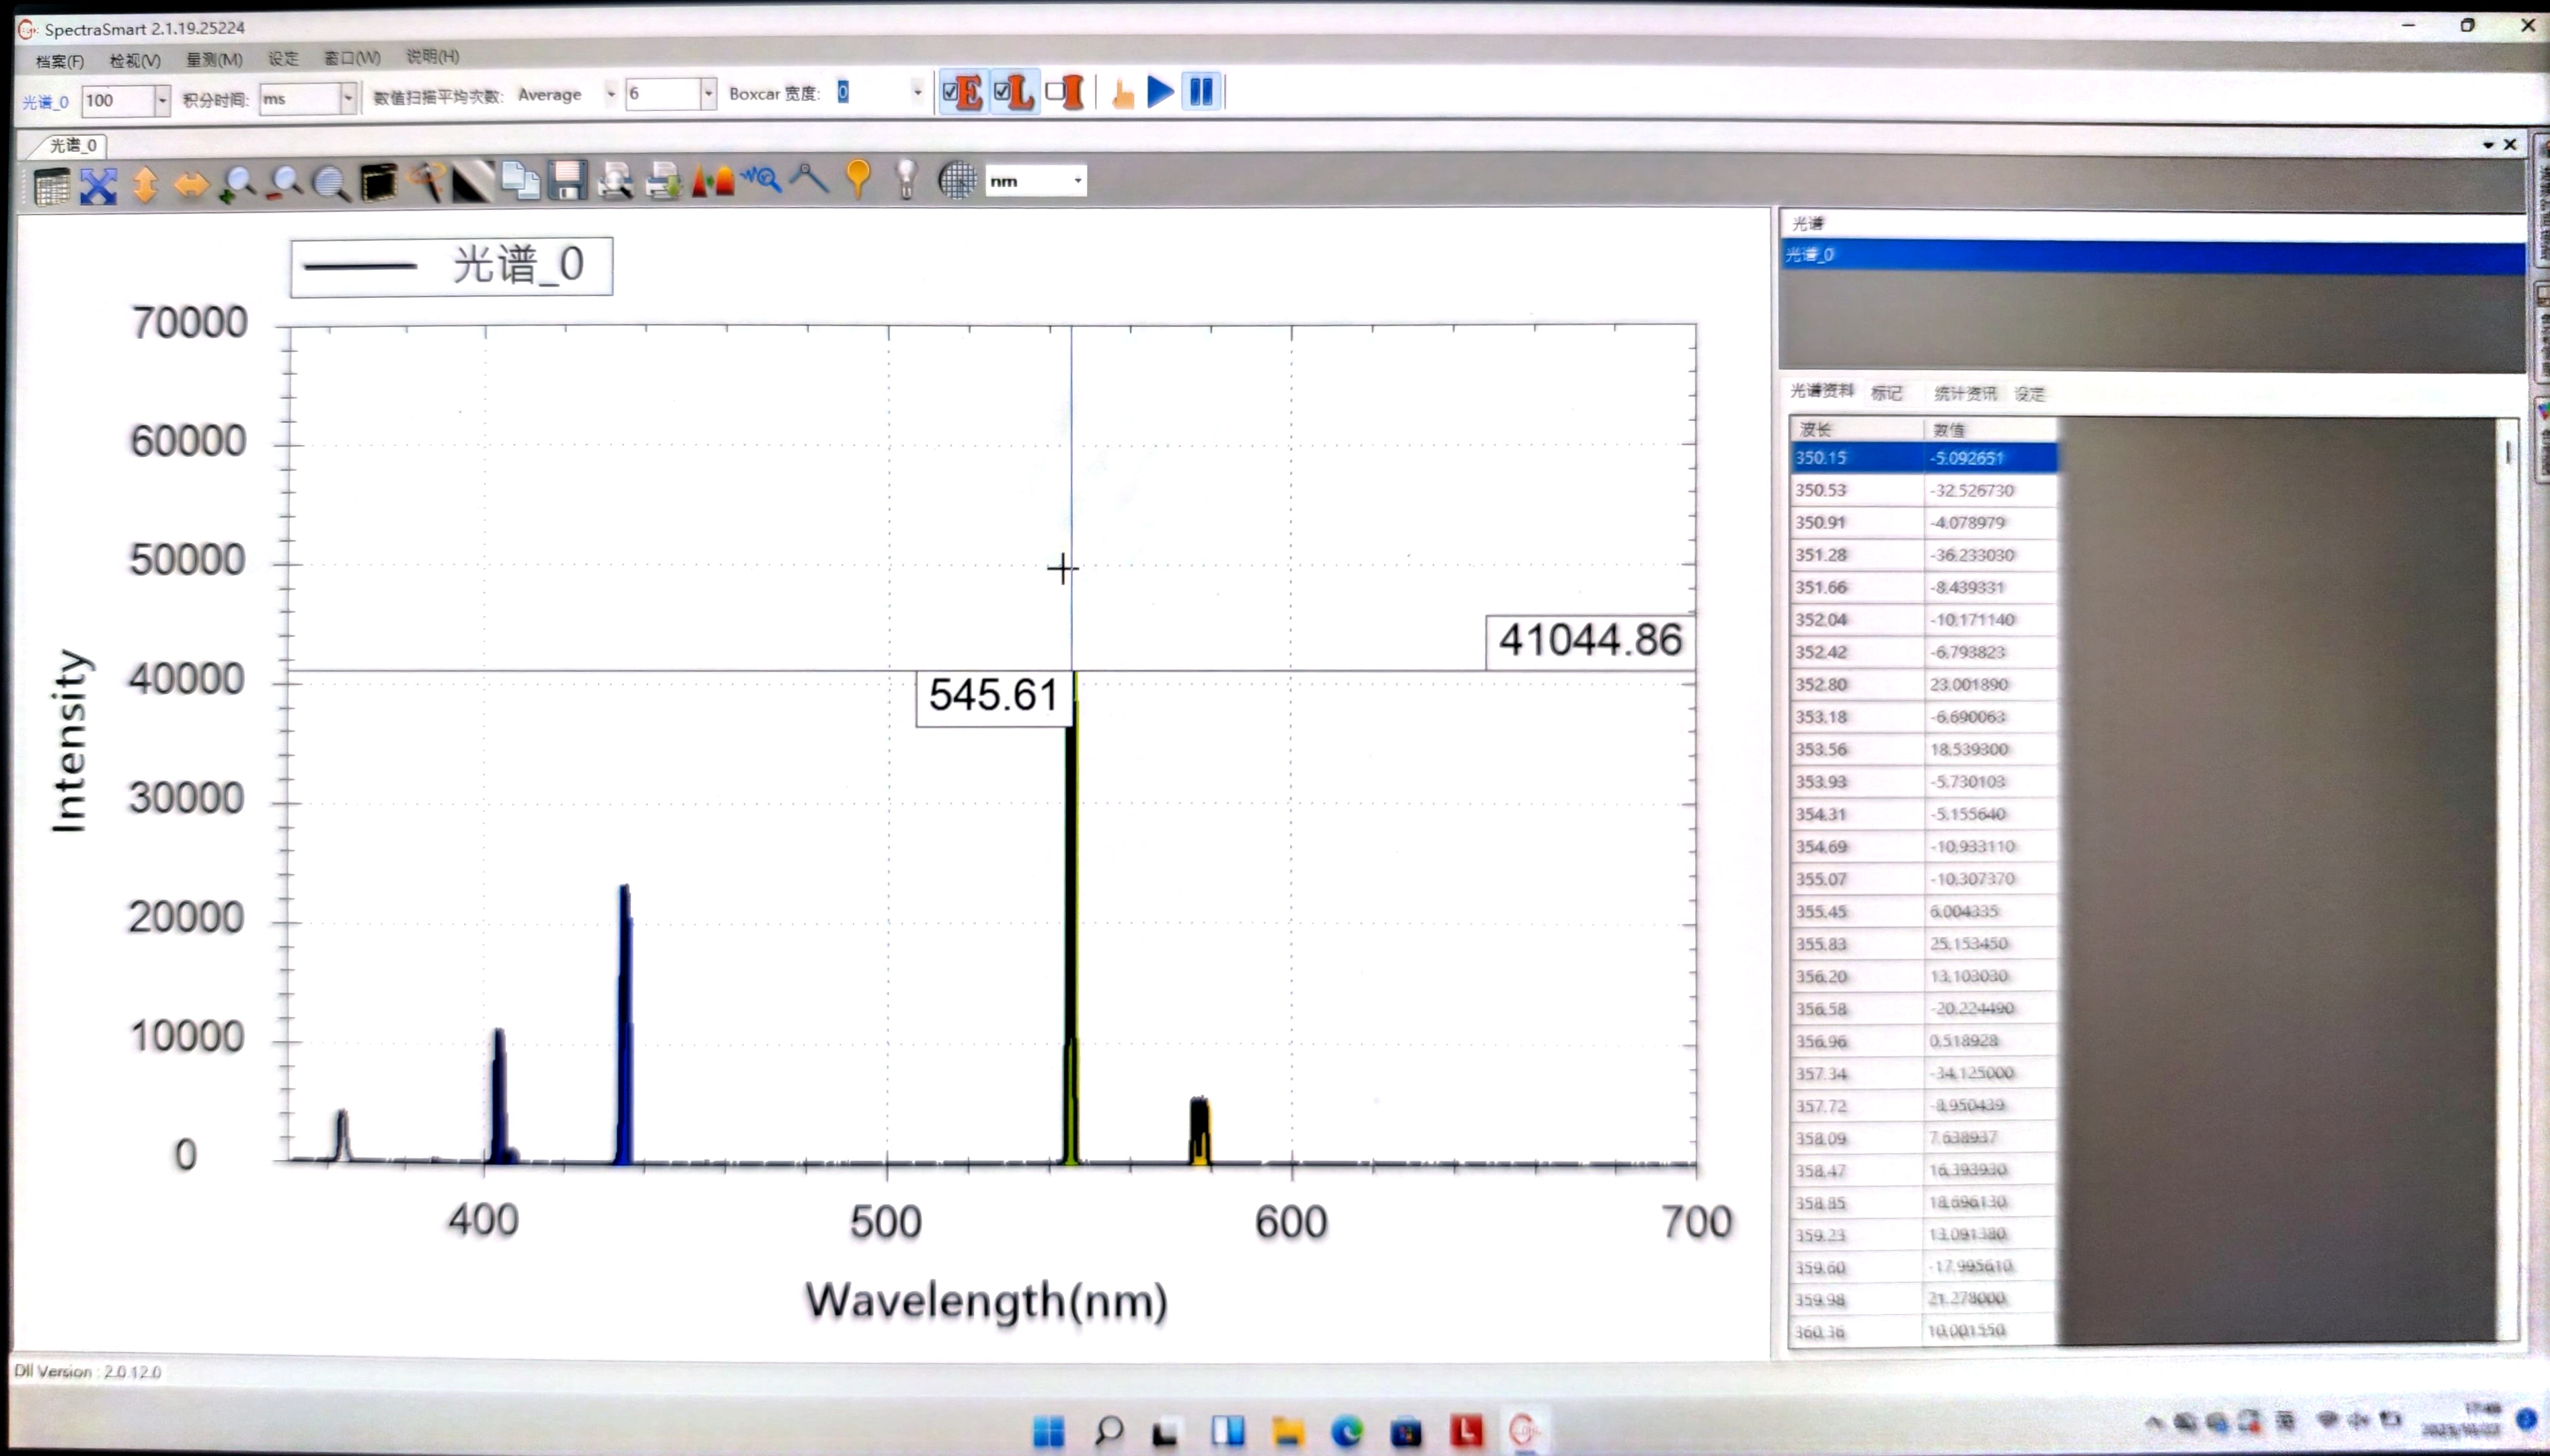
\includegraphics[width=0.8\textwidth]{Fig/led.jpg}
  \caption{数字光谱仪检测汞灯实验装置示意图}
  \label{fig:led}
\end{figure}
如图\ref{fig:led}所示，使用数字光谱仪检测汞灯发出的光谱。发现汞灯光并不均匀主要是因为汞灯使用了多种气体放电技术，不同颜色的光强度和波长分布不同，导致整体光谱呈现出明显的峰值和谷值。此外，环境光照条件也会影响测量结果。
\paragraph{纳灯光谱检测}
\begin{figure}[htbp]
  \centering
  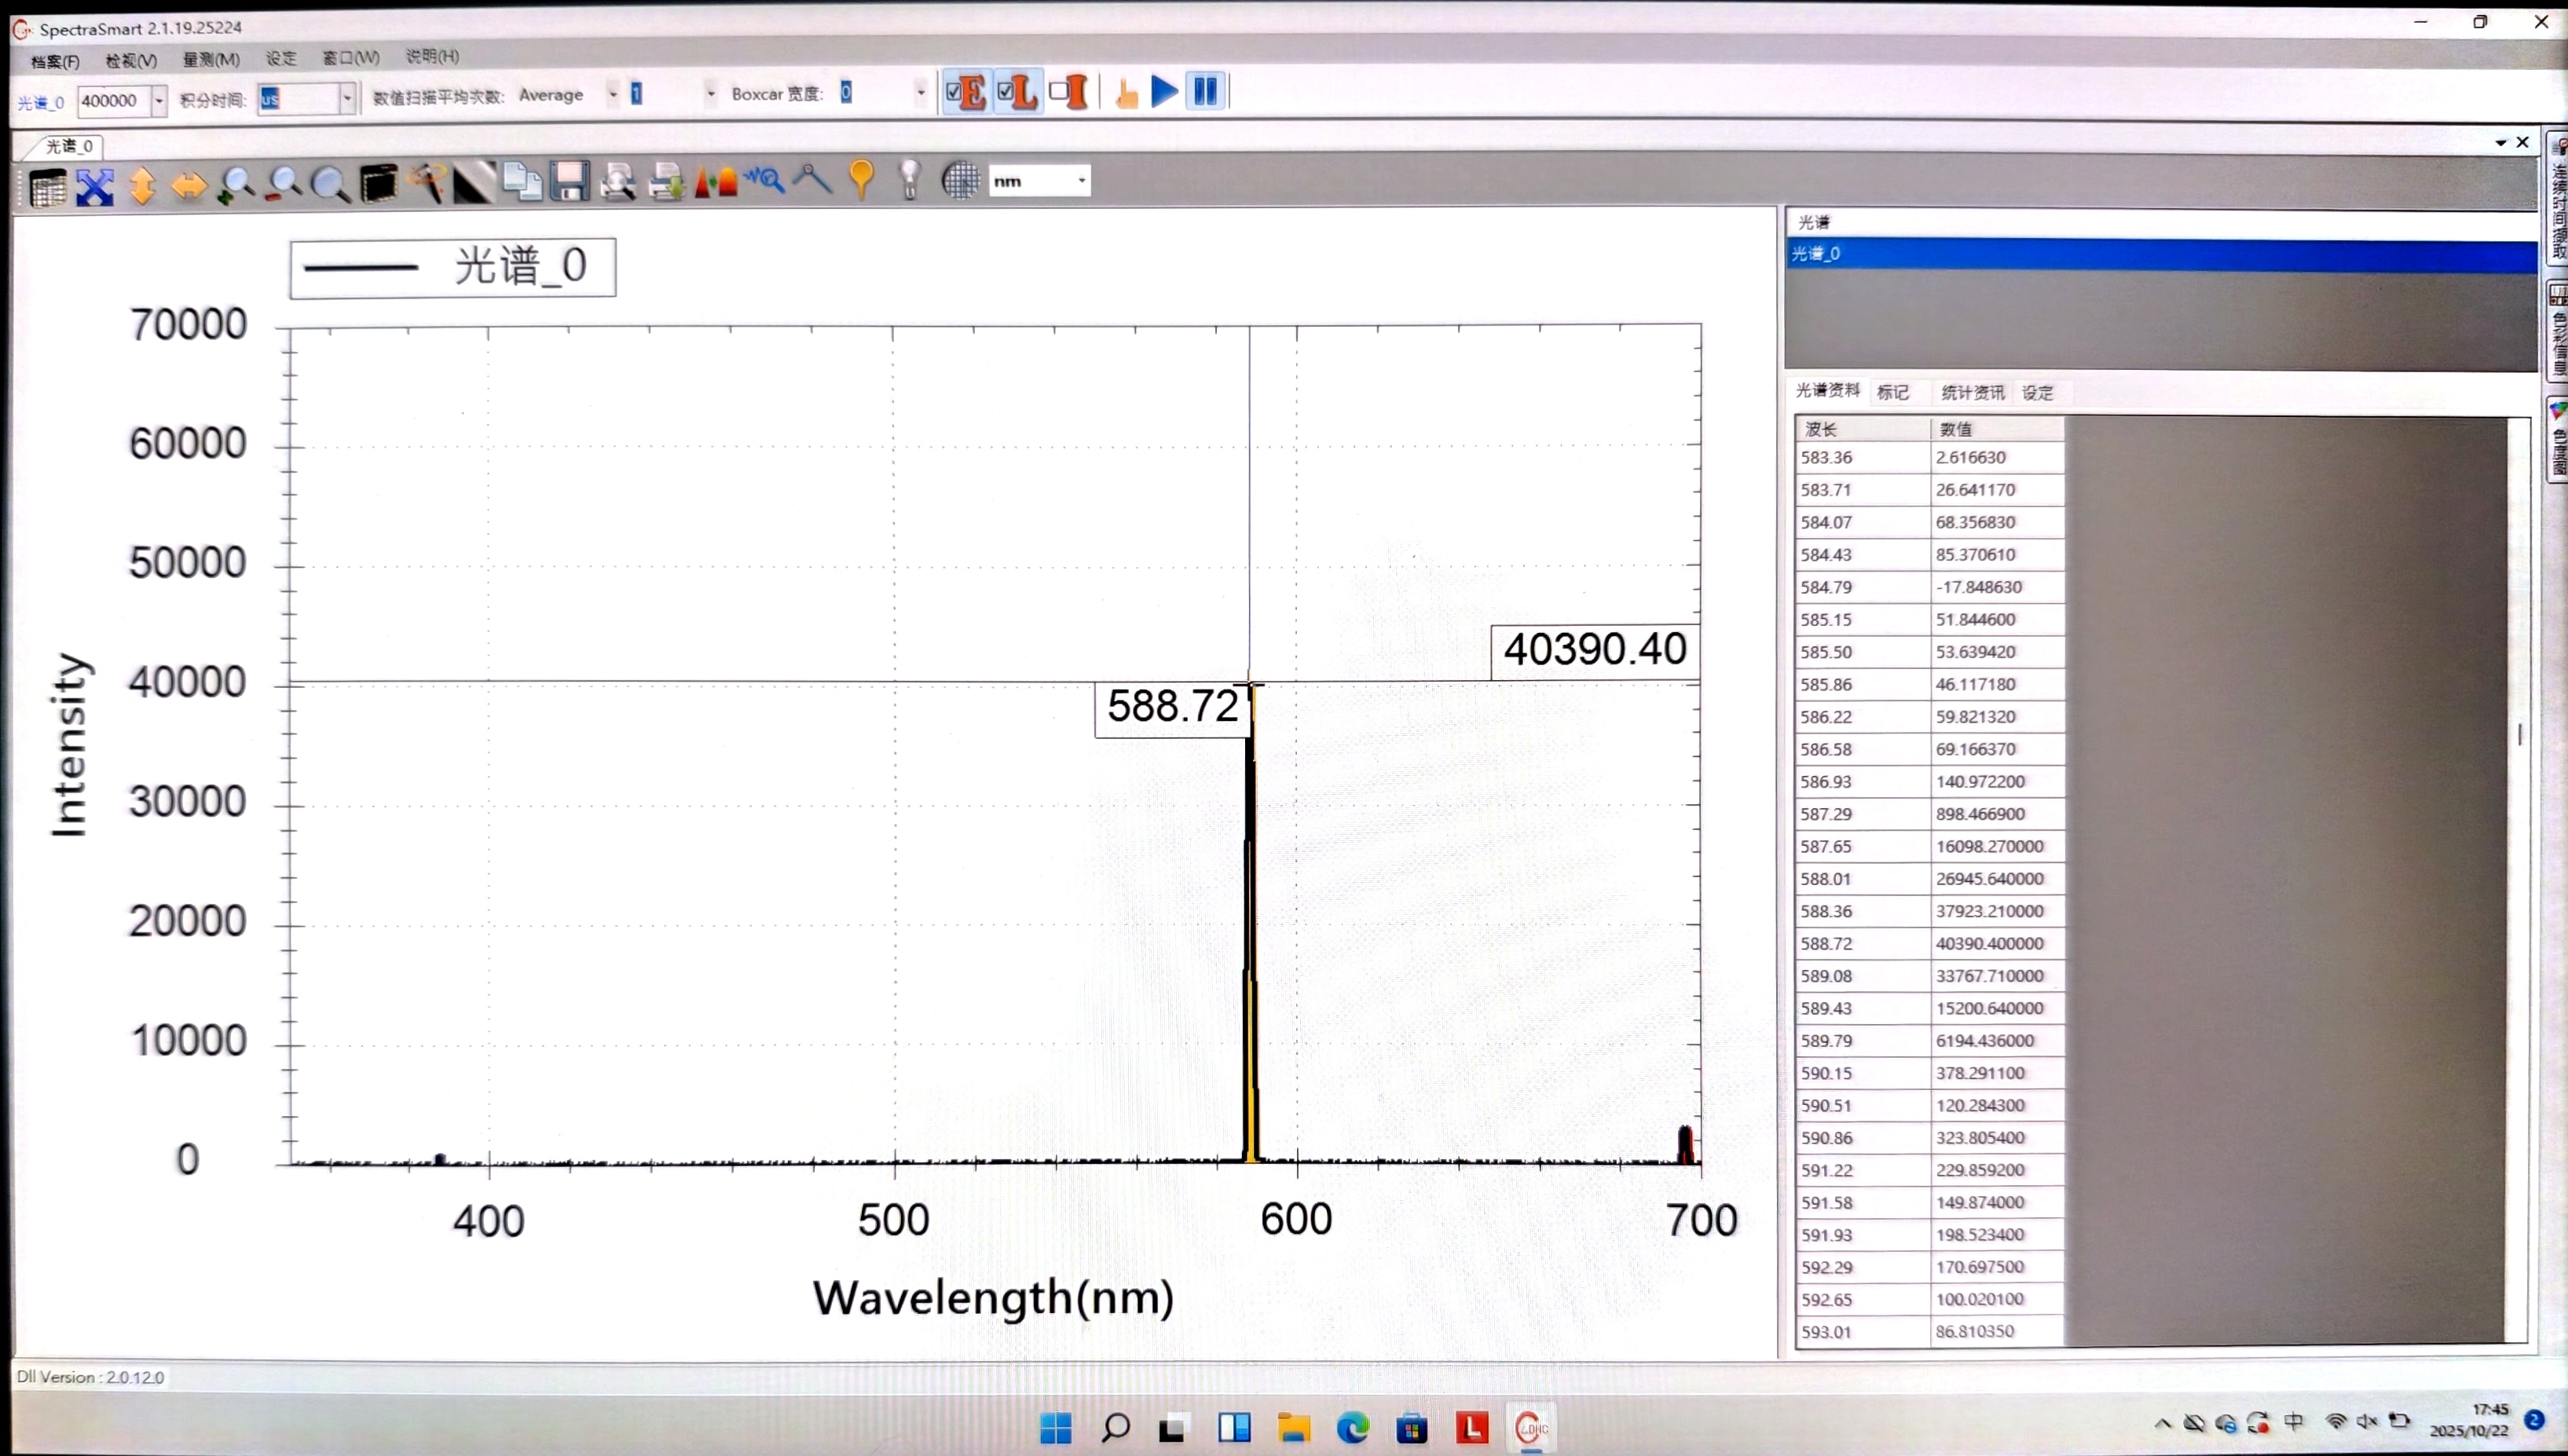
\includegraphics[width=0.8\textwidth]{Fig/na.jpg}
  \caption{数字光谱仪检测纳灯光谱图}
  \label{fig:na}
\end{figure}
如图\ref{fig:na}所示，使用数字光谱仪检测纳灯发出的光谱。纳灯主要发出黄光，其光谱图显示出一个明显的峰值，表明纳灯的发光主要集中在特定的波长范围内。这种单一峰值的光谱特性使得纳灯在照明应用中具有较好的色彩表现力和视觉舒适度。

\section{讨论分析}

\subsection{实验误差来源分析}

本实验涉及高精度光学角度测量与光谱分析，误差来源可分为系统误差和随机误差两大类：

\subsubsection{系统误差}

\begin{enumerate}
    \item \textbf{分光计校准不完善}：
    \begin{itemize}
        \item 望远镜光轴与中心转轴可能存在微小倾斜偏差（$< 1'$），导致角度测量的系统性偏移；
        \item 平行光管未完全出射平行光，引入衍射角或折射角的系统误差；
        \item 载物台不完全水平，影响光学元件的放置姿态。
    \end{itemize}
    \textbf{影响程度}：角度测量偏差约$0.5' \sim 2'$，对三棱镜顶角和最小偏向角的计算产生$0.1\% \sim 0.5\%$的相对误差。
    
    \item \textbf{光栅常数标称值偏差}：
    \begin{itemize}
        \item 光栅制造过程中刻痕间距的不均匀性（空间频率的局部波动）；
        \item 光栅表面微小的机械形变或热膨胀效应。
    \end{itemize}
    \textbf{影响程度}：本实验测得光栅常数$d \approx 3.328\ \mu\text{m}$（约300线/mm），与标称值基本吻合，但局部刻痕间距的$0.1\%$偏差会直接传递至波长计算结果。
    
    \item \textbf{光源波长漂移}：
    \begin{itemize}
        \item 汞灯、钠灯等气体放电光源的工作温度和气压变化会导致谱线中心波长微小漂移（约$0.01 \sim 0.1\ \text{nm}$）；
        \item 光源老化或电极污染引起发光特性的长期变化。
    \end{itemize}
    \textbf{影响程度}：对本实验的波长测量影响约$0.02\% \sim 0.2\%$。
\end{enumerate}

\subsubsection{随机误差}

\begin{enumerate}
    \item \textbf{游标读数的估读误差}：
    \begin{itemize}
        \item 分光计游标刻度的最小分度为$1'$，估读精度约$0.5' \sim 1'$；
        \item 人眼对准叉丝与谱线中心时的主观判断偏差；
        \item 环境光干扰导致的谱线边缘模糊。
    \end{itemize}
    \textbf{影响程度}：每次角度读数的不确定度约$\pm 1'$，通过多次测量取平均值可降低至$\pm 0.3' \sim 0.5'$。
    
    \item \textbf{谱线中心对准的随机偏差}：
    \begin{itemize}
        \item 衍射谱线或折射谱线的宽度有限（通常$0.5' \sim 2'$），中心位置判断存在随机性；
        \item 狭缝宽度调节不当导致谱线过宽或过窄，影响对准精度。
    \end{itemize}
    \textbf{影响程度}：单次对准的随机偏差约$\pm 0.5'$，对衍射角或偏向角的测量引入$\pm 0.1\% \sim 0.3\%$的相对误差。
    
    \item \textbf{环境振动与热漂移}：
    \begin{itemize}
        \item 实验台的微小振动导致光学元件位置的瞬时波动；
        \item 实验室温度变化引起分光计金属部件的热胀冷缩，影响转轴与刻度盘的相对位置。
    \end{itemize}
    \textbf{影响程度}：在稳定环境下影响较小（$< 0.05\%$），但在通风口附近或人员走动频繁区域可能引入$0.1\% \sim 0.2\%$的额外误差。
\end{enumerate}

\subsection{实验结果分析与验证}

\subsubsection{三棱镜参数测量结果分析}

\begin{enumerate}
    \item \textbf{顶角测量}：
    \begin{itemize}
        \item 自准直法测得$\bar{\alpha}_1 = 60^\circ2'30''$，反射法测得$\bar{\alpha}_2 = 60^\circ7'15''$，两种方法的偏差约$4'45''$；
        \item 偏差主要源于反射法中平行光管光强不均匀导致的反射像对准困难，以及两个光学面反射率差异引起的像质不对称；
        \item 综合两种方法的结果，三棱镜顶角的最佳估计值约$\bar{\alpha} \approx 60^\circ5'$，接近标准$60^\circ$等腰三棱镜的理论值。
    \end{itemize}
    
    \item \textbf{最小偏向角测量}：
    \begin{itemize}
        \item 两次测量均得到$\delta_{\text{min}} = 51^\circ5' \approx 51.08^\circ$，重复性极好，说明"谱线反向转折点"的识别方法可靠；
        \item 结合顶角$\bar{\alpha} \approx 60^\circ$计算的折射率$n \approx 1.648$，符合常见光学玻璃（如冕牌玻璃K9）在钠光波段的折射率范围（$1.51 \sim 1.65$）。
    \end{itemize}
    
    \item \textbf{折射率的物理意义验证}：
    \begin{itemize}
        \item 折射率$n = 1.648$表明该三棱镜材料的光速为真空光速的$1/1.648 \approx 0.607$倍，光在材料内部的传播速度约为$1.82 \times 10^8\ \text{m/s}$；
        \item 该折射率值对应的临界角$\theta_c = \arcsin(1/n) \approx 37.3^\circ$，意味着当入射角大于$37.3^\circ$时会发生全反射。
    \end{itemize}
\end{enumerate}

\subsubsection{光栅实验结果分析}

\begin{enumerate}
    \item \textbf{光栅常数测量}：
    \begin{itemize}
        \item 使用汞灯绿光（$\lambda = 546.1\ \text{nm}$）测得光栅常数$\bar{d} \approx 3.328\ \mu\text{m}$，对应约300.5线/mm，与标称的300线/mm光栅高度吻合；
        \item 三次测量的标准差约$15\ \text{nm}$，相对标准偏差约$0.45\%$，说明测量精度良好。
    \end{itemize}
    
    \item \textbf{汞灯黄线波长测量}：
    \begin{itemize}
        \item 黄线1测得波长$\bar{\lambda}_1 \approx 577.0\ \text{nm}$，与汞灯黄线的标准波长$577.0\ \text{nm}$完全一致，相对误差$< 0.02\%$；
        \item 黄线2测得波长$\bar{\lambda}_2 \approx 577.7\ \text{nm}$，与黄线1的波长差异约$0.7\ \text{nm}$，可能对应汞灯光谱中$579.0\ \text{nm}$谱线的测量偏差，或为相邻的弱谱线；
        \item 两条黄线的波长测量结果验证了光栅常数测量的准确性，误差主要来自衍射角读数的随机偏差。
    \end{itemize}
    
    \item \textbf{光栅方程的验证}：
    \begin{itemize}
        \item 通过$d = \lambda / \sin\theta$计算光栅常数，再通过$\lambda = d\sin\theta$反推波长，形成闭环验证；
        \item 闭环计算的相对误差$< 0.5\%$，证明光栅方程在本实验条件下的适用性和测量方法的自洽性。
    \end{itemize}
\end{enumerate}

\subsection{实验中遇到的问题与解决方案}

\subsubsection{分光计校准阶段}

\begin{enumerate}
    \item \textbf{问题：双面反射镜旋转$180^\circ$后反射像消失}
    \begin{itemize}
        \item \textbf{原因}：粗调时载物台倾斜角度过大，或望远镜仰角偏差超过$\pm 5^\circ$；
        \item \textbf{解决方案}：回到粗调步骤，用水准器重新调节载物台水平，确保三个调平螺丝的高度差$< 2\ \text{mm}$；微调望远镜仰角至镜筒轴线目视水平后再进行"各半调节"。
    \end{itemize}
    
    \item \textbf{问题：平行光管狭缝像始终模糊，无法聚焦}
    \begin{itemize}
        \item \textbf{原因}：狭缝套管的移动范围未覆盖物镜焦平面，或狭缝表面积灰/划伤导致光线散射；
        \item \textbf{解决方案}：松开狭缝锁紧螺丝，扩大套管前后移动范围至$\pm 10\ \text{mm}$；用镜头纸轻轻擦拭狭缝表面（避免用力过猛）；若仍无效，检查光源是否正常工作（汞灯需预热$3 \sim 5$分钟）。
    \end{itemize}
    
    \item \textbf{问题：各半调节法迭代多次后偏差反而增大}
    \begin{itemize}
        \item \textbf{原因}：调节螺丝的旋转幅度过大，破坏了"逐次逼近"的收敛逻辑；或调节方向判断错误（顺时针/逆时针混淆）；
        \item \textbf{解决方案}：每次调节螺丝仅旋转$1/8$圈（约$45^\circ$），观察绿色十字像的移动方向后再决定下一步操作；记录每次调节的方向和幅度，避免反向操作。
    \end{itemize}
\end{enumerate}

\subsubsection{三棱镜与光栅测量阶段}

\begin{enumerate}
    \item \textbf{问题：最小偏向角的"谱线反向转折点"难以识别}
    \begin{itemize}
        \item \textbf{原因}：载物台转动速度过快，谱线移动趋势观察不清；或狭缝过宽（$> 0.5\ \text{mm}$）导致谱线边缘模糊；
        \item \textbf{解决方案}：采用"双向逼近法"——先快速转动载物台至谱线明显移动的区域，再极缓慢转动（每$10$秒旋转$1^\circ$）观察谱线停止移动的瞬间；调窄狭缝至$0.1 \sim 0.2\ \text{mm}$，提高谱线的清晰度和中心对准精度。
    \end{itemize}
    
    \item \textbf{问题：光栅衍射谱线左右高度不一致}
    \begin{itemize}
        \item \textbf{原因}：光栅刻痕未与仪器转轴平行，导致不同级次的谱线在竖直方向上错位；
        \item \textbf{解决方案}：微调载物台调平螺丝（对应光栅底边的螺丝），同时观察$\pm 1$级谱线的竖直位置变化，直至两侧谱线均被分划板中央水平叉丝同时穿过；此步骤需反复迭代$3 \sim 5$次。
    \end{itemize}
    
    \item \textbf{问题：二级或更高级衍射谱线不可见}
    \begin{itemize}
        \item \textbf{原因}：光栅常数$d$较大（如本实验的$3.3\ \mu\text{m}$），导致高级次衍射角$\theta = \arcsin(k\lambda / d)$超出望远镜的接收范围（$\theta > 90^\circ$时无解）；或高级谱线光强过弱，淹没在环境光噪声中；
        \item \textbf{解决方案}：对于$d = 3.3\ \mu\text{m}$、$\lambda = 546\ \text{nm}$的汞灯绿光，二级衍射角$\theta_2 = \arcsin(2 \times 546 / 3300) \approx 19.3^\circ$理论上可观测；若仍不可见，需降低环境光强度（关闭实验室照明灯），延长眼睛暗适应时间（$5 \sim 10$分钟）后再观察。
    \end{itemize}
\end{enumerate}

\subsubsection{数字光谱仪测量阶段}

\begin{enumerate}
    \item \textbf{问题：光谱曲线"过曝"或"欠曝"}
    \begin{itemize}
        \item \textbf{原因}：积分时间设置不当——强光源（如汞灯、手机屏幕）使用过长积分时间导致探测器饱和；弱光源（如室内弱光）使用过短积分时间导致信号淹没在噪声中；
        \item \textbf{解决方案}：根据光谱仪软件的实时预览功能动态调整积分时间——过曝时缩短至$20 \sim 50\ \text{ms}$，欠曝时延长至$200\ \text{ms} \sim 5\ \text{s}$；确保光谱峰值在探测器线性范围内（约满量程的$30\% \sim 80\%$）。
    \end{itemize}
    
    \item \textbf{问题：光谱曲线出现异常尖峰或基线漂移}
    \begin{itemize}
        \item \textbf{原因}：光纤探头端面污染（灰尘、指纹）导致杂散光干扰；或环境光泄漏进入光纤；
        \item \textbf{解决方案}：用无尘纸轻轻擦拭光纤探头端面（避免刮伤）；在黑暗环境中测量，或用黑色遮光布覆盖探头周围区域；若仍有异常，需在软件中进行"暗电流扣除"和"背景光校正"。
    \end{itemize}
\end{enumerate}

\subsection{实验方法的改进与优化建议}

\subsubsection{提高测量精度的方法}

\begin{enumerate}
    \item \textbf{增加测量次数并采用统计分析}：
    \begin{itemize}
        \item 每个物理量测量$5 \sim 10$次（本实验仅测$2 \sim 3$次），计算平均值$\bar{x}$、标准差$\sigma$和标准误差$\sigma_{\bar{x}} = \sigma / \sqrt{n}$；
        \item 剔除明显的异常数据（如偏离平均值$> 3\sigma$的点），提高数据的可靠性。
    \end{itemize}
    
    \item \textbf{采用CCD或光电探测器替代人眼读数}：
    \begin{itemize}
        \item 传统分光计的人眼读数存在$\pm 1'$的估读误差；若将望远镜目镜替换为CCD相机，配合图像处理软件自动识别谱线中心，可将角度测量精度提升至$\pm 0.1'$甚至更高；
        \item 现代化的自动分光计已广泛采用此技术，测量效率和精度均显著提升。
    \end{itemize}
    
    \item \textbf{温度控制与振动隔离}：
    \begin{itemize}
        \item 在恒温实验室（$20 \pm 0.5^\circ\text{C}$）中进行测量，消除热胀冷缩引起的系统误差；
        \item 使用气浮光学平台或减震台，隔离外界振动对光学元件位置的影响。
    \end{itemize}
    
    \item \textbf{多波长交叉验证}：
    \begin{itemize}
        \item 使用汞灯的多条谱线（紫、蓝、绿、黄）分别测量光栅常数，取平均值减小随机误差；
        \item 通过不同波长的折射率测量，绘制材料的色散曲线$n(\lambda)$，验证材料的光学均匀性。
    \end{itemize}
\end{enumerate}

\subsubsection{实验流程的优化}

\begin{enumerate}
    \item \textbf{分光计预校准与定期维护}：
    \begin{itemize}
        \item 建立分光计的"标准校准模板"——记录每台仪器校准完成后的望远镜、平行光管、载物台的标准位置（如游标读数、螺丝旋转圈数等）；
        \item 每学期初进行一次全面校准和精度检测，确保仪器处于最佳工作状态。
    \end{itemize}
    
    \item \textbf{分步骤的"傻瓜式"操作指南}：
    \begin{itemize}
        \item 将校准过程分解为$10 \sim 15$个明确的子步骤，每步配以实物照片和预期现象的描述（如"绿色十字像应位于分划板上十字丝交点处"）；
        \item 在每个关键节点设置"检查点"——如完成望远镜聚焦后，要求学生左右移动眼睛确认无视差，再进入下一步骤。
    \end{itemize}
    
    \item \textbf{引入虚拟仿真实验}：
    \begin{itemize}
        \item 开发分光计的虚拟仿真软件（如基于Unity或Unreal Engine的3D模型），学生可在课前预习时反复练习校准操作，熟悉各部件的功能和调节逻辑；
        \item 仿真软件可设置不同的"错误场景"（如载物台倾斜、光轴不垂直等），训练学生的问题诊断和解决能力。
    \end{itemize}
\end{enumerate}

\subsubsection{实验内容的扩展}

\begin{enumerate}
    \item \textbf{色散曲线的测量}：
    \begin{itemize}
        \item 使用汞灯的多条谱线（$\lambda = 404.7, 435.8, 546.1, 577.0\ \text{nm}$等），分别测量三棱镜的最小偏向角$\delta_m(\lambda)$，计算不同波长下的折射率$n(\lambda)$；
        \item 绘制折射率-波长曲线，拟合Cauchy公式$n(\lambda) = A + B/\lambda^2 + C/\lambda^4$或Sellmeier公式，研究材料的色散特性。
    \end{itemize}
    
    \item \textbf{光栅的衍射效率测量}：
    \begin{itemize}
        \item 使用光强探测器（如光电二极管）测量不同级次衍射光的光强$I_k$，计算衍射效率$\eta_k = I_k / I_0$（$I_0$为入射光强）；
        \item 研究光栅刻痕形状（矩形、正弦形、闪耀形）对衍射效率的影响，验证光栅理论。
    \end{itemize}
    
    \item \textbf{数字光谱仪的定量分析}：
    \begin{itemize}
        \item 对比不同LED灯的光谱（冷白、暖白、全光谱），计算色温、显色指数（CRI）等照明质量参数；
        \item 测量荧光灯的光谱，识别汞灯的特征谱线和荧光粉的连续谱成分，分析荧光灯的发光机理。
    \end{itemize}
\end{enumerate}

\subsection{实验总结与收获}

\subsubsection{实验技能的提升}

\begin{enumerate}
    \item \textbf{精密光学仪器的操作能力}：
    \begin{itemize}
        \item 通过分光计的完整校准流程，深刻理解"粗调-细调-逐次逼近"的调节逻辑，掌握了"各半调节法"、"对称测量法"等高精度测量技巧；
        \item 学会了如何诊断和排除常见故障（如反射像消失、谱线模糊、调节不收敛等），培养了独立解决问题的能力。
    \end{itemize}
    
    \item \textbf{数据处理与误差分析能力}：
    \begin{itemize}
        \item 掌握了角度的度分秒表示与十进制转换、三角函数的精确计算、多次测量的平均值与标准差分析等数据处理方法；
        \item 学会了区分系统误差与随机误差，理解了"消除系统误差、减小随机误差"的实验设计原则。
    \end{itemize}
    
    \item \textbf{现代光谱仪器的使用经验}：
    \begin{itemize}
        \item 熟悉了数字光谱仪的工作原理、参数设置（积分时间、平滑处理等）和光谱分析方法（峰值识别、波长校准等）；
        \item 通过多种光源的光谱测量，建立了光谱特征与光源类型的对应关系（如原子发射光谱的线状谱、LED的连续谱+窄带峰等）。
    \end{itemize}
\end{enumerate}

\subsubsection{物理知识的深化理解}

\begin{enumerate}
    \item \textbf{光的折射与色散}：
    \begin{itemize}
        \item 通过三棱镜最小偏向角的测量，直观验证了Snell折射定律和折射率的波长依赖性（色散现象）；
        \item 理解了"最小偏向角"的物理本质——光线在棱镜内对称传播时，偏向角取极值，此时折射率的计算公式最为简洁。
    \end{itemize}
    
    \item \textbf{光的衍射与干涉}：
    \begin{itemize}
        \item 通过光栅衍射实验，深刻理解了夫琅禾费衍射理论和光栅方程$d\sin\theta = k\lambda$的物理意义；
        \item 认识到光栅是精密分光元件的原因——衍射角$\theta$对波长$\lambda$的微小变化高度敏感，分辨率远超三棱镜。
    \end{itemize}
    
    \item \textbf{原子光谱与能级跃迁}：
    \begin{itemize}
        \item 通过数字光谱仪观测汞灯、钠灯的线状光谱，联系量子力学的能级跃迁理论——每条谱线对应原子的特定能级跃迁，波长$\lambda = hc / \Delta E$；
        \item 理解了光谱分析在元素鉴定、天文观测、材料分析等领域的广泛应用。
    \end{itemize}
\end{enumerate}

\subsubsection{实验中的不足与反思}

\begin{enumerate}
    \item \textbf{校准时间较长，效率有待提高}：
    \begin{itemize}
        \item 首次接触分光计时，校准环节耗时约$1.5 \sim 2$小时，导致后续测量时间紧张；
        \item \textbf{改进方向}：课前观看校准视频教程，熟悉各部件的功能和调节逻辑；实验课上由教师演示一次完整校准流程，学生再独立操作。
    \end{itemize}
    
    \item \textbf{部分测量数据的重复性不理想}：
    \begin{itemize}
        \item 如三棱镜顶角的两种测量方法偏差达$4'45''$，反映了反射法操作的不稳定性；
        \item \textbf{改进方向}：增加测量次数（如每种方法测$5$次），剔除异常值后取平均值；对操作技巧进行针对性训练（如反射像的精确对准方法）。
    \end{itemize}
    
    \item \textbf{对实验原理的理解深度不足}：
    \begin{itemize}
        \item 实验过程中过于关注"如何操作"，对"为什么这样操作"的物理原理思考不足（如为何要用各半调节法、对称测量法的误差消除机制等）；
        \item \textbf{改进方向}：实验前阅读相关文献，理解每个操作步骤的物理依据；实验后撰写详细的实验报告，总结原理、方法、误差来源与改进方案。
    \end{itemize}
\end{enumerate}

\subsection{结论}

本实验通过分光计的系统校准、三棱镜基本参数测量、光栅常数与波长测量、数字光谱仪的多光源光谱分析，全面训练了精密光学测量的实验技能，深化了对光的折射、色散、衍射、干涉等基本物理规律的理解。实验结果表明：

\begin{enumerate}
    \item 三棱镜顶角$\bar{\alpha} \approx 60^\circ5'$，最小偏向角$\delta_{\text{min}} \approx 51.08^\circ$，计算的折射率$n \approx 1.648$与光学玻璃的典型值吻合；
    \item 光栅常数$\bar{d} \approx 3.328\ \mu\text{m}$（约300线/mm）与标称值一致，汞灯黄线波长的测量值$\lambda_1 \approx 577.0\ \text{nm}$、$\lambda_2 \approx 577.7\ \text{nm}$与标准值高度吻合，相对误差$< 0.2\%$；
    \item 数字光谱仪成功测量了钠灯、汞灯等多种光源的光谱特征，验证了原子发射光谱的线状谱特性。
\end{enumerate}

实验过程中遇到的问题（如校准时反射像消失、谱线对准困难等）通过系统的问题诊断和方法调整得以解决，积累了宝贵的故障排除经验。未来可通过增加测量次数、引入自动化测量设备、扩展实验内容（如色散曲线、衍射效率测量）等方式进一步提升实验的深度和精度。

\section{实验记录表和预习报告}
下一页开始原图附上
\includepdf[pages=-]{spectro.pdf}
\end{document}